\chapter{Practical Considerations on the Topological Correctness of Marching Cubes 33}
\label{chap:mc33}

Isosurface extraction techniques can be divided into two classes according to their topological guarantees, namely, consistency or correctness. Topologically \emph{consistent} techniques produce surfaces that are piecewise-linear (PL) manifolds (\emph{i.e.}, crack-free surfaces), except at the boundary of the domain. To-pologically \emph{correct} techniques produce a PL-manifold homeomorphic to the surface induced by a given interpolant, such as the trilinear interpolant. Although there are many topologically \emph{consistent} MC-based techniques, only a handful are topologically \emph{correct}. Marching Cubes 33 is one of the first MC-based algorithms that aim to preserve the topology of the trilinear interpolant.

Topological correctness increases the complexity of isosurface extraction algorithms. 
The many isosurface configurations possible for a given interpolant in a cubic grid makes both the algorithm and its implementation a challenging task. 
%
As algorithms and implementations become more complex, issues may be overlooked and remain hidden in the multitude of (pseudo-) lines of code.
%
Throughout years of research, it has been shown that some supposedly topologically correct techniques, including \mc, have issues that prevent correctness  \cite{Etiene:2012:TVI:2197070.2197097, lopes:tvcg:2003, newman:candg:2006}. 
%
In particular, the work of Etiene \emph{et al.} \cite{Etiene:2012:TVI:2197070.2197097} shows that the \mc{} implementation by Lewiner \emph{et al.} \cite{lewiner:impl,Lewiner:2003}, fails to produce topologically correct isosurfaces. 
%
Alas, the authors \emph{do not} provide an explanation for the problem source, let alone fix the problem. 
%
They only provide cases that are mishandled by \mc{} and a conjecture regarding  the root of one of the observed flaws.
%
As we studied the \mc{} implementation, we realized that the source of the problem was not merely implementation bugs but the core ideas behind the implemented algorithm.  
%
In this work, we address issues with Chernyaev's original algorithm, its extension, and its implementation. 
%
Our work closes an existing gap in the topological correctness of Marching Cubes 33.
 
 The subtleties involved in the correctness of isosurface extraction techniques are sometimes difficult to grasp in the ordinary paper medium. Both the geometry and topology inside grid voxels are often complex and challenging to understand,  study and replicate ({\em e.g.}, see Figures 9 and 10 in~\cite{Nielson03onmarching}).  As an attempt to bridge this gap, we build on recent efforts towards \emph{executable papers}~\cite{Koop:2011tv, Tohline:2010jn}. Executable papers extend the traditional paper/digital counterpart by including tools that allow readers to interact, explore and verify experiments more easily.  In this chapter, we use executable papers to increase the reproducibility of our results.
 %
 
Our contributions, which have a practical nature, are the following:
\begin{itemize}
\item We explain and address three algorithmic issues and one non-trivial implementation issue with Marching Cubes 33. In particular, we solve an issue with the core \mc{} disambiguation procedure that, as far as we know, has not been addressed elsewhere. Hence, we close an existing gap in the \mc{} literature.
\item We make our results reproducible. CrowdLabs~\cite{Tohline:2010jn} and Vistrails \cite{Freire:2006va} are used to create an executable paper that can reproduce the results shown in the following sections.
\item We provide datasets that  can be used to verify the correctness of any topologically correct isosurface extraction technique.
\end{itemize}
A by-product of this work is a thorough analysis of both the \mc{} algorithm and its implementation that can be used by anyone interested in  the use or development of correct isosurface extraction algorithms based on \mc{}. The results of our efforts are materialized into an extended version of the \mc{} implementation \cite{lewiner:impl}, henceforth called Corrected-MC33 (\cmc).

This work is organized as follows. Section \ref{sec:preliminaries} reviews key aspects related to the Marching Cubes 33 algorithm. Section \ref{experiments_setup} explains how experiments that uncovered problems in both \mc{} algorithm and implementation were conducted. The details of the problems found are shown in Section \ref{erros_cause:chernyaev} and the solutions are presented in Section \ref{sec:solution}. Section \ref{sec:real-world} shows the results of applying algorithm with different topological guarantees to real-world datasets.

%============================================================================================



\section{Related Work}
\label{related_work1}

Soon after the publication of the MC algorithm, the quest for a topologically correct isosurface extraction technique began. A number of approaches were proposed for dealing with cracks, face ambiguity, and, lastly, interior ambiguity.
%
D\"urst \cite{Durst88} was the first to point out that some MC cases allow multiple triangulations. A consequence of this is that MC does not always generate topologically consistent surfaces. This problem arises due to the \emph{ambiguity problem}; and
the Asymptotic Decider \cite{Nielson:1991:ADR:949607.949621} provides a simple and elegant solution to face ambiguity.

The ambiguity problem also occurs in the interior of a voxel. Natarajan \cite{Natarajan:1994:GTC:205424.205429}  was the first to address this problem by adding four new cases to the standard MC triangulation table (subcases of cases 3, 4, 6, and 7). To find the correct subcases, the author proposed a disambiguation procedure based on both face and interior critical points. Nevertheless,  the method misses the possibility of two interior critical points in case 7, consequently the proposed algorithm may generate a surface with the incorrect topology~\cite{10.1109/TVCG.2009.10, newman:candg:2006}.

Using a different approach, Chernyaev \cite{Chernyaev95marchingcubes} extended the original MC table to 33 cases -- hence \mc{}; this extension included all the subcases for each ambiguous case. He used the Asymptotic Decider and a new interior ambiguity test to discriminate among subcases. Lewiner \emph{et al.} \cite{Lewiner:2003} provided a practical open-source implementation of the Chernyaev algorithm. It is worth noting that some of the configurations shown in Chernyaev's work~\cite{Chernyaev95marchingcubes} may have been inspired by personal communication with Nielson \cite{Nielson03onmarching}.
%
Matveyev~\cite{Matveyev99} introduced an isosurface technique that is also based on an extended table and used the intersections of isosurfaces with cube diagonals to determine the correct case. 

Lopes and Brodlie \cite{lopes:tvcg:2003} extended the tests proposed by Natarajan. The goals of the work are threefold: i) extract topologically correct isosurfaces; ii) produce geometrically accurate isosurface; iii) allow continuity with respect to changes in threshold and data.  Nevertheless, as in Natarajan's work, the method missed the possibility of two interior critical points in case 7~\cite{lopes:tvcg:2003}.
%
Cignoni \emph{et al.}~\cite{Cignoni2000399} also used the test proposed by Natarajan to reconstruct topologically correct isosurfaces.
%
The work of Theisel \cite{CGF:CGF00563} uses B\'ezier patches to build $G^1$ continuous isosurfaces that are topologically correct.  Nielson \cite{Nielson03onmarching} lists all possible cases of a trilinear interpolant inside a cubic grid and builds a topologically correct MC using a three stage algorithm for surface polygonization. 

The past two decades have also produced a number of isosurface techniques that are not MC-based. Dual Contouring~\cite{Ju:2002:DCH:566654.566586} (DC) is a robust, crack-free, isosurface extraction technique that works on the dual grid. Several improvements over Dual Contouring have been proposed: Schaefer \emph{et al.}~\cite{Schaefer:2007:MDC:1263130.1263312} address the issue of non-manifold surfaces generated by DC; Varadhan \emph{et al.}~\cite{Varadhan:2003:FSI:1081432.1081458} combine a signed distance field with DC to reconstruct details such as thin features; and Zhang \emph{et al.}~\cite{Zhang:2004:DCT:1032664.1034486} use DC for topology-preserving simplification of isosurfaces. Note that none of these techniques are intended to preserve the topology of the trilinear interpolant. Dey and Levine~\cite{Dey07} presented an algorithm that computes a Delaunay triangulation based on the intersection between the isosurface and the 3D Voronoi diagram. Another paradigm for isosurface extraction is the advancing front method. Advancing front algorithms build a triangulated surface by progressively adding triangles to an implicit surface~\cite{Hartmann98}, possibly creating several fronts that are simultaneously advanced one triangle at a time.  A number of extensions have been proposed for advancing front techniques \cite{Schreiner06, CGF:CGF972, Silva:1998:GCA:288692.288717}. 

In the following sections, we focus on \mc{}. Note that, although many of the  algorithms presented previously are topologically consistent, only a handful of them are topologically correct~\cite{Chernyaev95marchingcubes, Dey07}. Also, the implementation of a topologically correct isosurface extraction algorithm is non-trivial.
Hence, once the algorithm is implemented, topological guarantees, both  consistency and correctness, may be lost because of algorithm or implementation issues, as shown in the work of Etiene \emph{et al.}~\cite{Etiene:2012:TVI:2197070.2197097}. 
%
Although it has been ten years since the publication of \mc{}, we believe it is important to correct a mistake in the algorithm that has gone unnoticed since Chernyaev published it almost 20 years ago. In this work we aim to close an existing gap in the \mc{} literature. Furthermore, we aim not only to provide a correct algorithm but verify that our modified implementation is faithful to the correct algorithm.  We explain the issues and propose solutions for both algorithm and implementation. 
%
We note that ``\mc{}'' may refer to either the Marching Cubes 33 \emph{algorithm} presented in Chernyaev's work \cite{Chernyaev95marchingcubes} or its \emph{implementation}, as in Lewiner \emph{et al.}  \cite{Lewiner:2003} depending on the context.

%============================================================================================

\section{Preliminaries}
\label{sec:preliminaries}

In this section we present the notation that will be used throughout this chapter. We also briefly review the main concepts behind Chernyaev's algorithm and Lewiner \emph{et al.}'s improvements to it. 
%
Let $G$ be a rectilinear grid with scalar values associated with each vertex $x_j \in G$. Let $g:\mathbb{R}^3 \rightarrow \mathbb{R}$ be a piecewise-trilinear interpolation function defined on $G$. Given an isovalue $\lambda$,  the isosurface $S_\lambda$ is defined as the set of points for which $g(x)=\lambda$. For each voxel $v_i \subset G$, and $x \in v_i$, $g(x) = g_i(x)$ where $g_i$ is the trilinear interpolant inside the cubic cell $v_i$. 

The output of MC-based algorithms is a piecewise-linear mesh $M_\lambda$, and we say that an algorithm and its implementation are \emph{topologically correct} if $M_\lambda$ is homeomorphic to $S_\lambda$. Without loss of generality, we assume that $\lambda = 0$, and thus $S_\lambda = S_0 = S$. We say that a point $x$ is \emph{positive} (\emph{negative}) if $g(x) > 0$ ($g(x) < 0$). 

Given a voxel $v_i$, and a cutting-plane $P$ parallel to one of $v_i$'s faces, define  $f_i:\mathbb{R}^2 \rightarrow \mathbb{R}$ as the bilinear interpolant along $P$. Note that $f_i(x) = g_i(x)$ for $x \in P$. Throughout the text, we deal with a single voxel $v$; thus, we omit the subscript $i$. We also assume that $v$ and $P$ are defined in the domains  $[0,1]^3$ and $[0,1]^2$, respectively.

\begin{figure}[b]
     \centering
     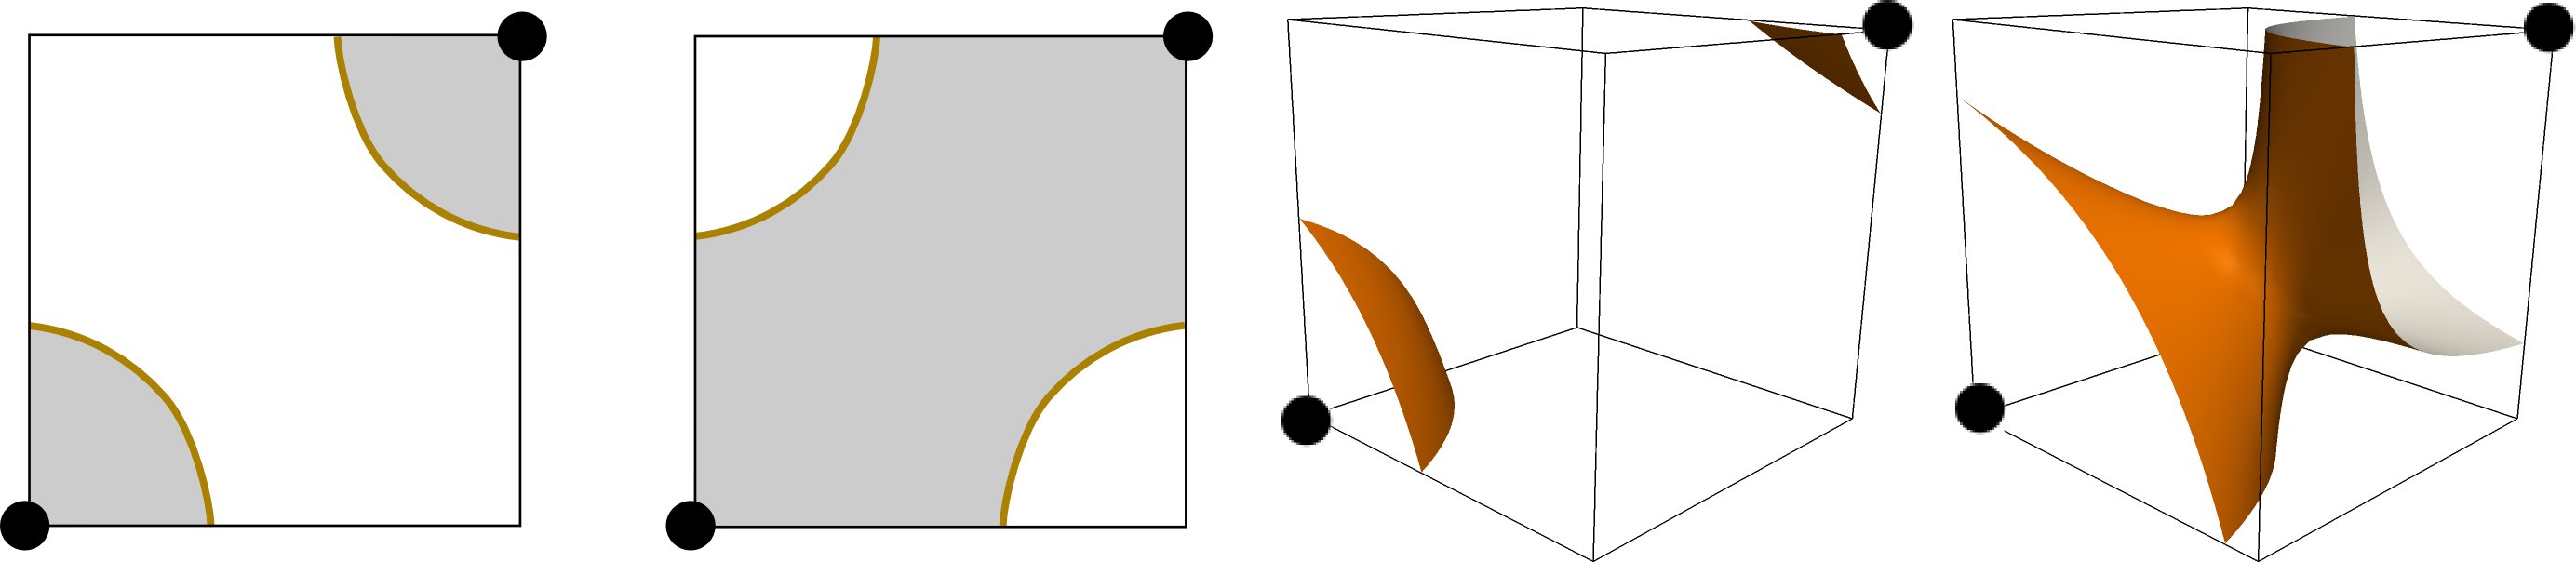
\includegraphics[width=1\linewidth]{chapter4/figures/ambiguity.png}
     \caption{Left: case 4 ambiguity. The interior ambiguity test proposed by Chernyaev is used choose the correct configuration.Right: face ambiguity. The Asymptotic Decider  is used to resolve the ambiguity.}
     \label{ambiguity}
\end{figure}
 
\begin{figure}[t]
     \centering
     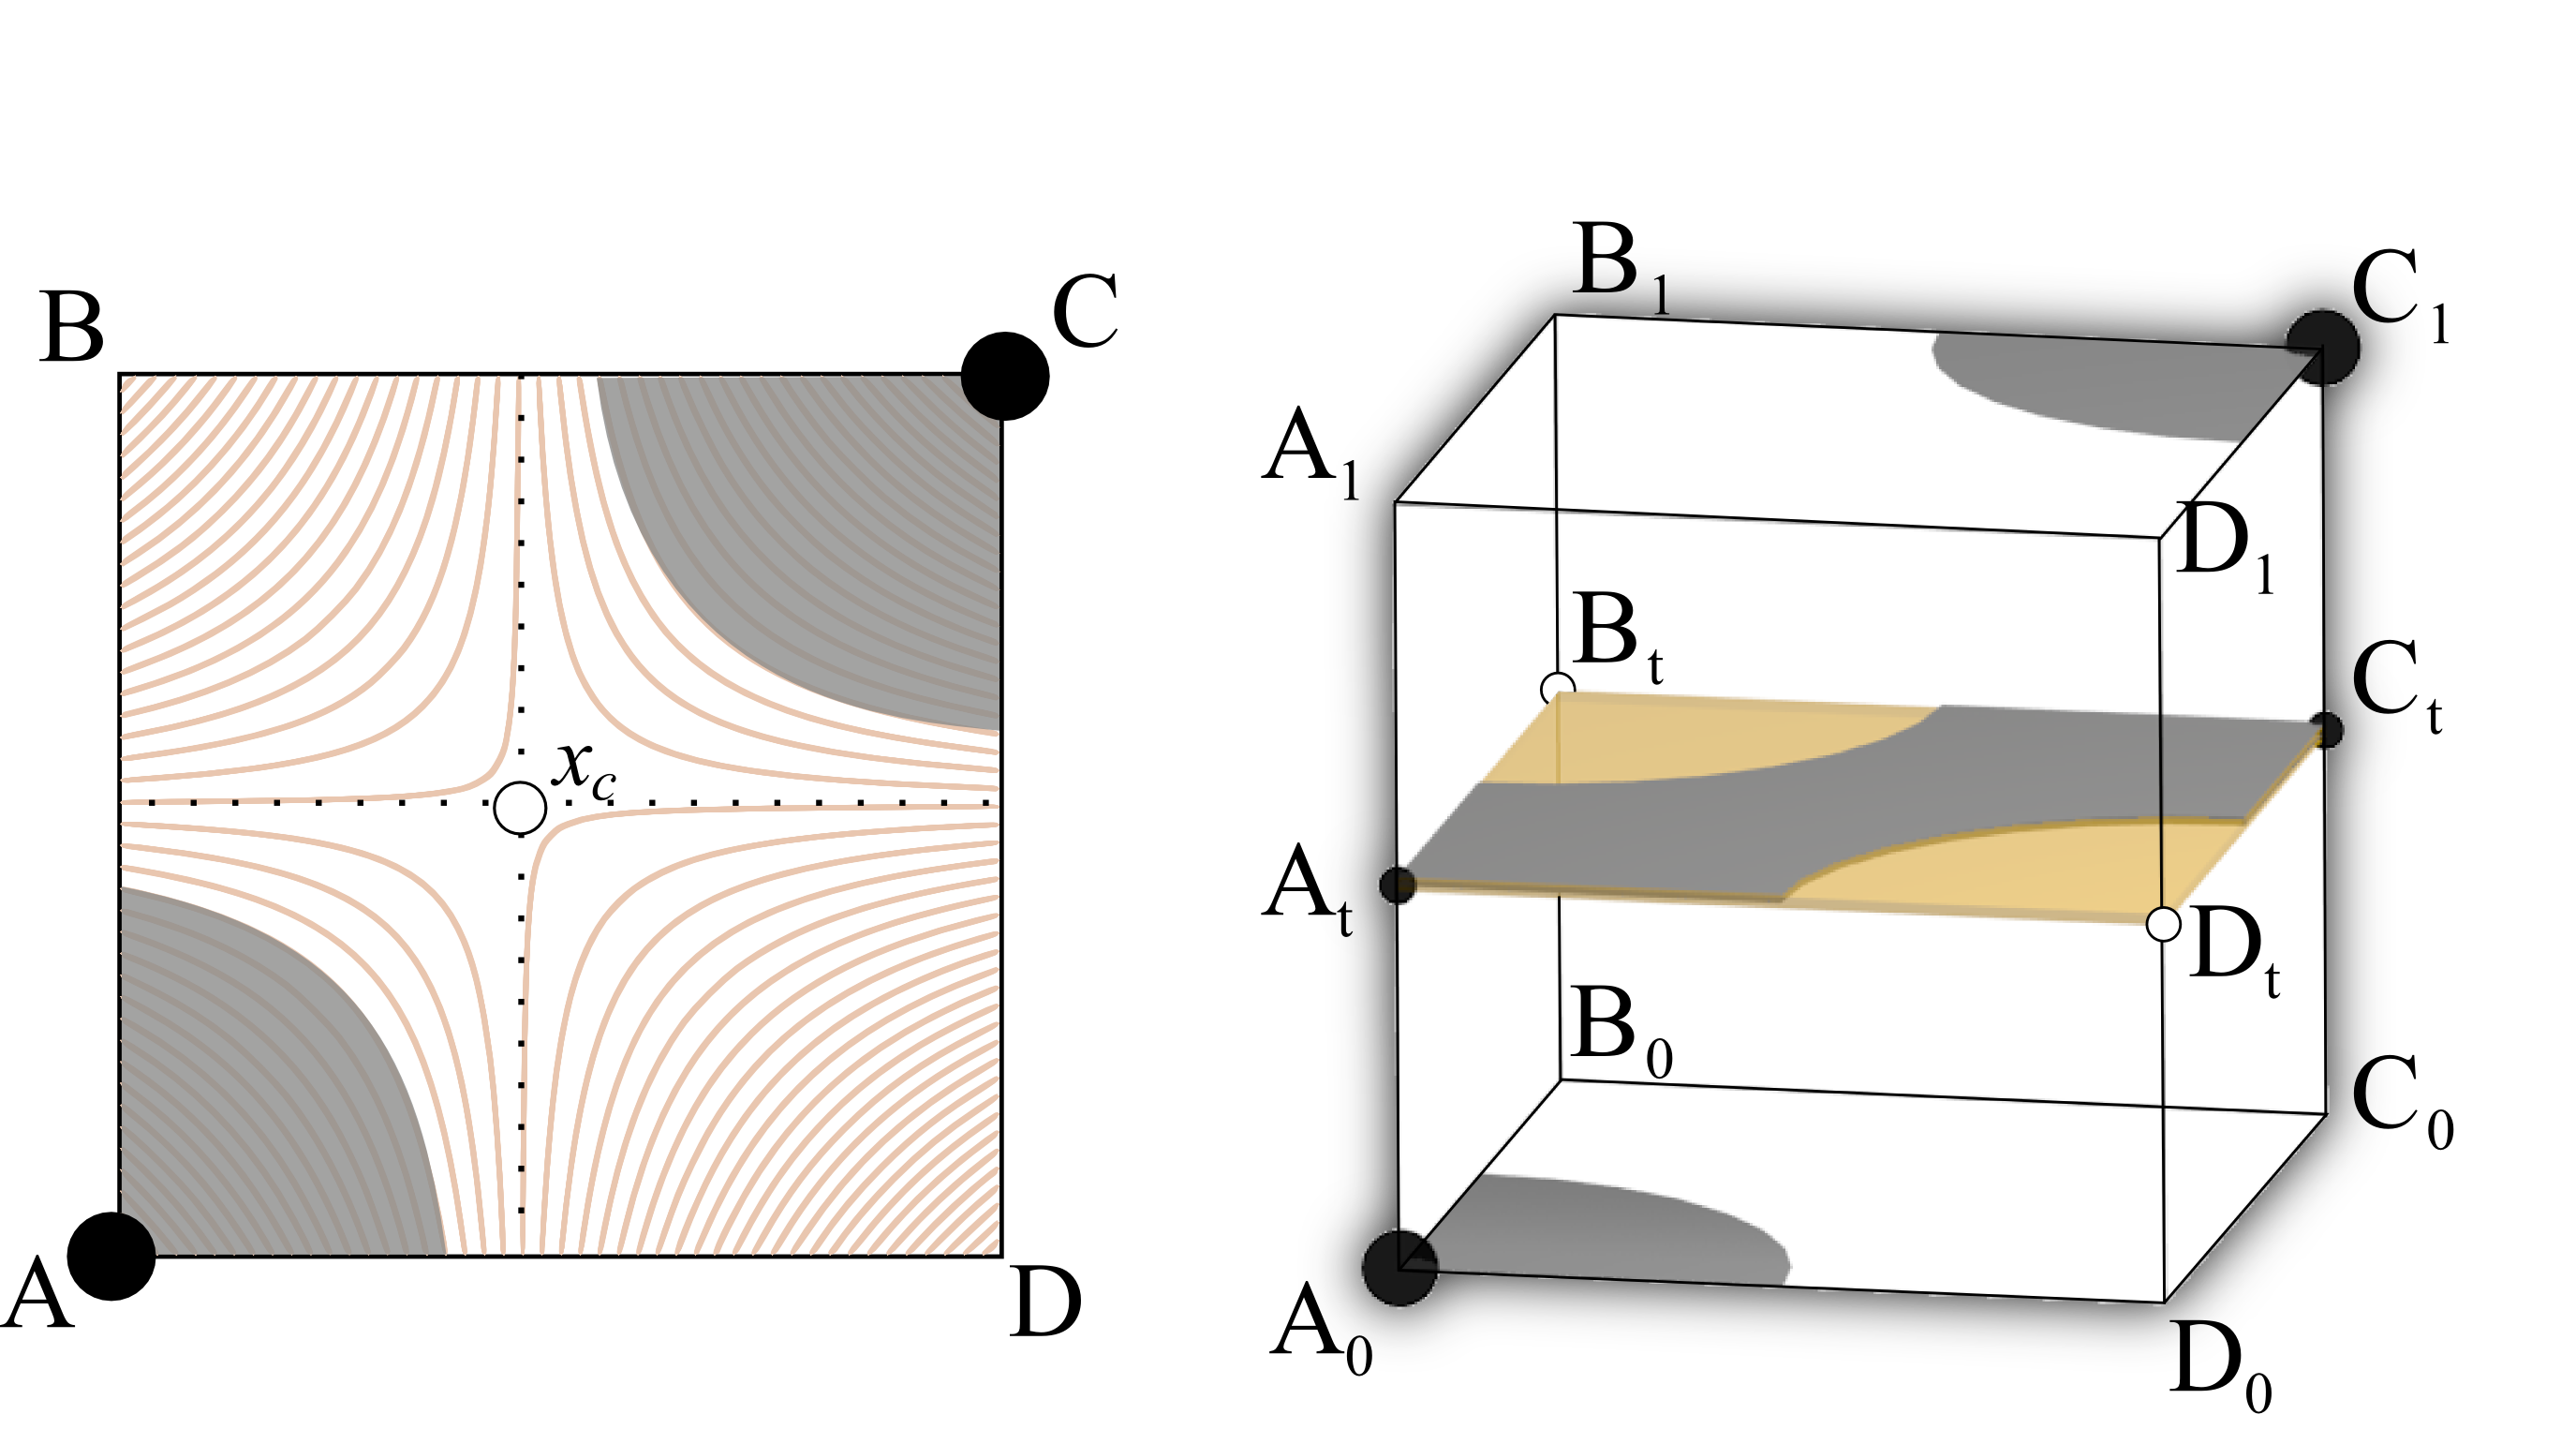
\includegraphics[width=0.65\linewidth]{chapter4/figures/cut-plane-fig.png}
     \caption{Asymptotic Decider (left) and \mc{} interior ambiguity test for MC case 4 (right). The gray areas represent regions with positive scalar values, and the capital letters represent the scalar value at each vertex. In the left image, we observe that $f(x_c) < 0$, where $x_c$ is the saddle point position. Positive areas will be connected if $f(x_c) > 0$. The orange squared plane shown in the right image represents the cutting-plane. The goal of the \mc{} algorithm is to find a cutting-plane such that the gray areas in the top and bottom planes are joined in the interior.}
     \label{interior_ambiguity}
\end{figure}


\subsection{Chernyaev's \mc{}}

The two pillars of Marching Cubes 33's topological correctness are Nielson and Hamann's Asymptotic Decider and Chernyaev's interior ambiguities test; together these solve the face ambiguity and interior ambiguity problems in the Marching Cubes 33 algorithm.
%
A face ambiguity occurs when face vertices have alternating signs. That is, one face diagonal is positive (both vertices are positive) and the other is negative (both vertices are negative). In this case, the signs of the face vertices are insufficient to determine the correct way to triangulate the isosurface. Similarly, an interior ambiguity occurs when the signs of the cube vertices are insufficient to determine the correct surface triangulation, \emph{i.e.}, when multiple triangulations are possible for the same cube configuration (see Figure \ref{ambiguity}).

The idea behind the Asymptotic Decider is to verify the face saddle sign and compare it to the sign on the face vertices. A positive saddle means that the positive face vertices are connected; consequently, the positive face vertices are separated if the face saddle point is negative (see Figure \ref{interior_ambiguity}). To compute the face saddle sign, the saddle point position $x_c$ must be computed~\cite{Chernyaev95marchingcubes}:
\begin{eqnarray}
x_c & = & \left( \frac{A - D}{A+C-B-D}, \frac{A - B}{A+C-B-D} \right), \label{eq:saddle_position}
\end{eqnarray}
where $A$, $B$, $C$ and $D$ are the scalar values at the face vertices (see Figure \ref{interior_ambiguity}).
%
The sign of $x_c$ can easily be checked by replacing Equation \eqref{eq:saddle_position} into the bilinear interpolant:
\begin{eqnarray}
f(x_c) & = & \frac{AC - BD}{A+C-B-D}.\label{eq:saddle_value}
\end{eqnarray}
For an ambiguous face, assuming $A$, $C$ positive and $B$ and $D$ negative, the denominator of the Equation \eqref{eq:saddle_value} is always positive (see Figure \ref{interior_ambiguity}). Then, the face ambiguity is solved by evaluating the sign of the numerator of $f(x_c)$.

Due to the interior ambiguity, the Asymptotic Decider alone cannot solve the topological correctness problem. Chernyaev uses the idea behind the Asymptotic Decider to solve the interior ambiguity problem. The proposed test uses a  sweeping cutting-plane to evaluate the behavior of the trilinear interpolant inside the cube.

Given a cube with an ambiguous configuration, define the scalar values at the base and top planes as $A _{0}$, $B_{0}$, $C_{0}$, $D_{0}$ and $A _{1}$, $B_{1}$, $C_{1}$, $D_{1}$, respectively (see Figure \ref{interior_ambiguity}).  Let $A_{0}$ and $C_{1}$, the vertices to be tested, be positive. Observe that, although $A_{0}$ and $C_{1}$ belong to opposite cube faces, they can be connected through the cube interior. In other words, there may exist a path from $A_0$ to $C_1$ passing through the voxel interior for which all points belonging to that path are positive. To determine whether $A_0$ and $C_1$ are connected, Chernyaev begins by observing that the saddle points at the top and base cube faces are negative, \emph{i.e.}, Equation \eqref{eq:saddle_value} is negative at the bottom and top faces. Since the denominator is positive, it follows that:
 %
\begin{eqnarray}
A_0C_0 - B_0D_0 &<& 0 \label{eq:condition1}\\
A_1C_1 - B_1D_1 &<& 0 \label{eq:condition2}.
\end{eqnarray}

Then, if there is a plane cutting the cube such that its saddle point is positive, it means that there is a positive area crossing the cube,  \emph{i.e.}  the positive vertices are connected inside the cube.  In other words, the Chernyaev interior test searches for a $t$ for which:
\begin{eqnarray}
F(t) = A_tC_t-B_tD_t &>& 0. \label{eq:chernyaev_test}
\end{eqnarray}
This can be achieved by solving a second order equation in $t$. Replacing $X_t = X_0 + (X_1-X_0)t$,  $X \in \{A, B, C, D\}$ and $t \in [0,1]$ in Equation \eqref{eq:chernyaev_test} one obtains a second order equation in $t$:
\begin{eqnarray}
F(t) &=& A_tC_t-B_tD_t\\
       &=& a t^2 + b t + c  \label{eq:disambiguation},
\end{eqnarray}
where $a$, $b$, and $c$ are functions of $A, B, C,$ and $D$ (see \ref{app:counter-example}). Chernyaev concludes that positive vertices $A_0$ and $C_1$ are connected through the cube interior if: 
\begin{enumerate}
\item $a < 0$;
\item $t_{\mathrm{max}} = -b / 2a \in (0,1)$; 
\item $F(t_{\mathrm{max}}) > 0$. 
\end{enumerate}
If one of the above conditions fails, the positive vertices are separated.

\subsection{Lewiner \emph{et al.}'s \mc{}}

Lewiner \emph{et al.}~\cite{Lewiner:2003} proposed a modification of Chernyaev's interior test. In this modification, they use an alternative method for computing the height plane $t$ for most ambiguous cases. For cases  6, 7, 12, and 13, the authors compute the height $t$ based on the barycenter of the end vertices of an edge $e$ (a cube edge intersected by the isosurface) weighted by the values of the scalar field on these vertices (see \cite{Lewiner:2003} for details). In practice, the implementation uses:
\begin{eqnarray}
t_{\mathrm{alt}} &=& \frac{V_{0}}{V_{0} - V_{1}},\label{eq:alternative}
\end{eqnarray}
where $V_{0}$ and $V_{1}$ are the scalar values at the vertices of $e$. Note that this is equivalent to finding the intersection point between the isosurface $S$ and $e$. The authors keep the structure of the test proposed by Chernyaev, but condition (i) is not used, and condition (ii) is always true because $e$ is an edge intersected by the isosurface; consequently, $t_{alt} \in (0,1)$.

Section \ref{erros_cause:chernyaev} explains why the algorithm proposed by Chernyaev and its modified version proposed by Lewiner \emph{et al.} may fail to extract surfaces that are topologically correct. In the following section, we present the tools we use to detect, debug, and reproduce the issues found in the \mc{} algorithm and its implementation. The full Marching Cubes table can be found in the works of Chernyaev \cite{Chernyaev95marchingcubes} and Lewiner \emph{et al.}\cite{Lewiner:2003}.


\section{Experiments setup}
\label{experiments_setup}

We begin by investigating the source of topological problems in the \mc{} implementation~\cite{Etiene:2012:TVI:2197070.2197097}.
%
The topological issues described were obtained by systematically stress-testing the implementation over many topological configurations using the verification framework proposed in Etiene \emph{et al.}~\cite{Etiene:2012:TVI:2197070.2197097}. These authors' algorithm can be summarized as follows.
%
(I) A random scalar field $G$ is built by uniformly sampling scalar values in the range $[-1,1]$ for each $x_j \in G$.
%
(II) The \emph{expected topological invariants} are obtained directly from $S$, {\em i.e.}, without extracting the isosurface of interest. The topological invariants used are the Euler characteristic $\chi(S)$ and the Betti numbers $\beta_k(S)$. 
%
(III) The \mc{} implementation is used to extract a piecewise linear mesh $M$, and its invariants $\chi(M)$ and $\beta_k(M)$ are computed.
%
(IV) Lastly, the pairs of topological invariants $\{\chi(S)$, $\chi(M)\}$ and $\{\beta_k(S), \beta_k(M)\}$ are compared. A mismatch indicates that a problem has occurred. Nevertheless,  as the authors note, a match between invariants does not imply a bug-free code~\cite{Etiene:2012:TVI:2197070.2197097}. The verification process does not prove the absence of bugs but only increases one's confidence in its correctness.
%
In this chapter, we exploit the fact that when the expected and obtained surfaces are not homeomorphic, a counterexample is given in the form of a scalar field $G$ and a mesh $M$. We use this information to find and correct errors in \mc{}.

\subsection{Reproducibility}

\begin{figure}[b]
     \centering
    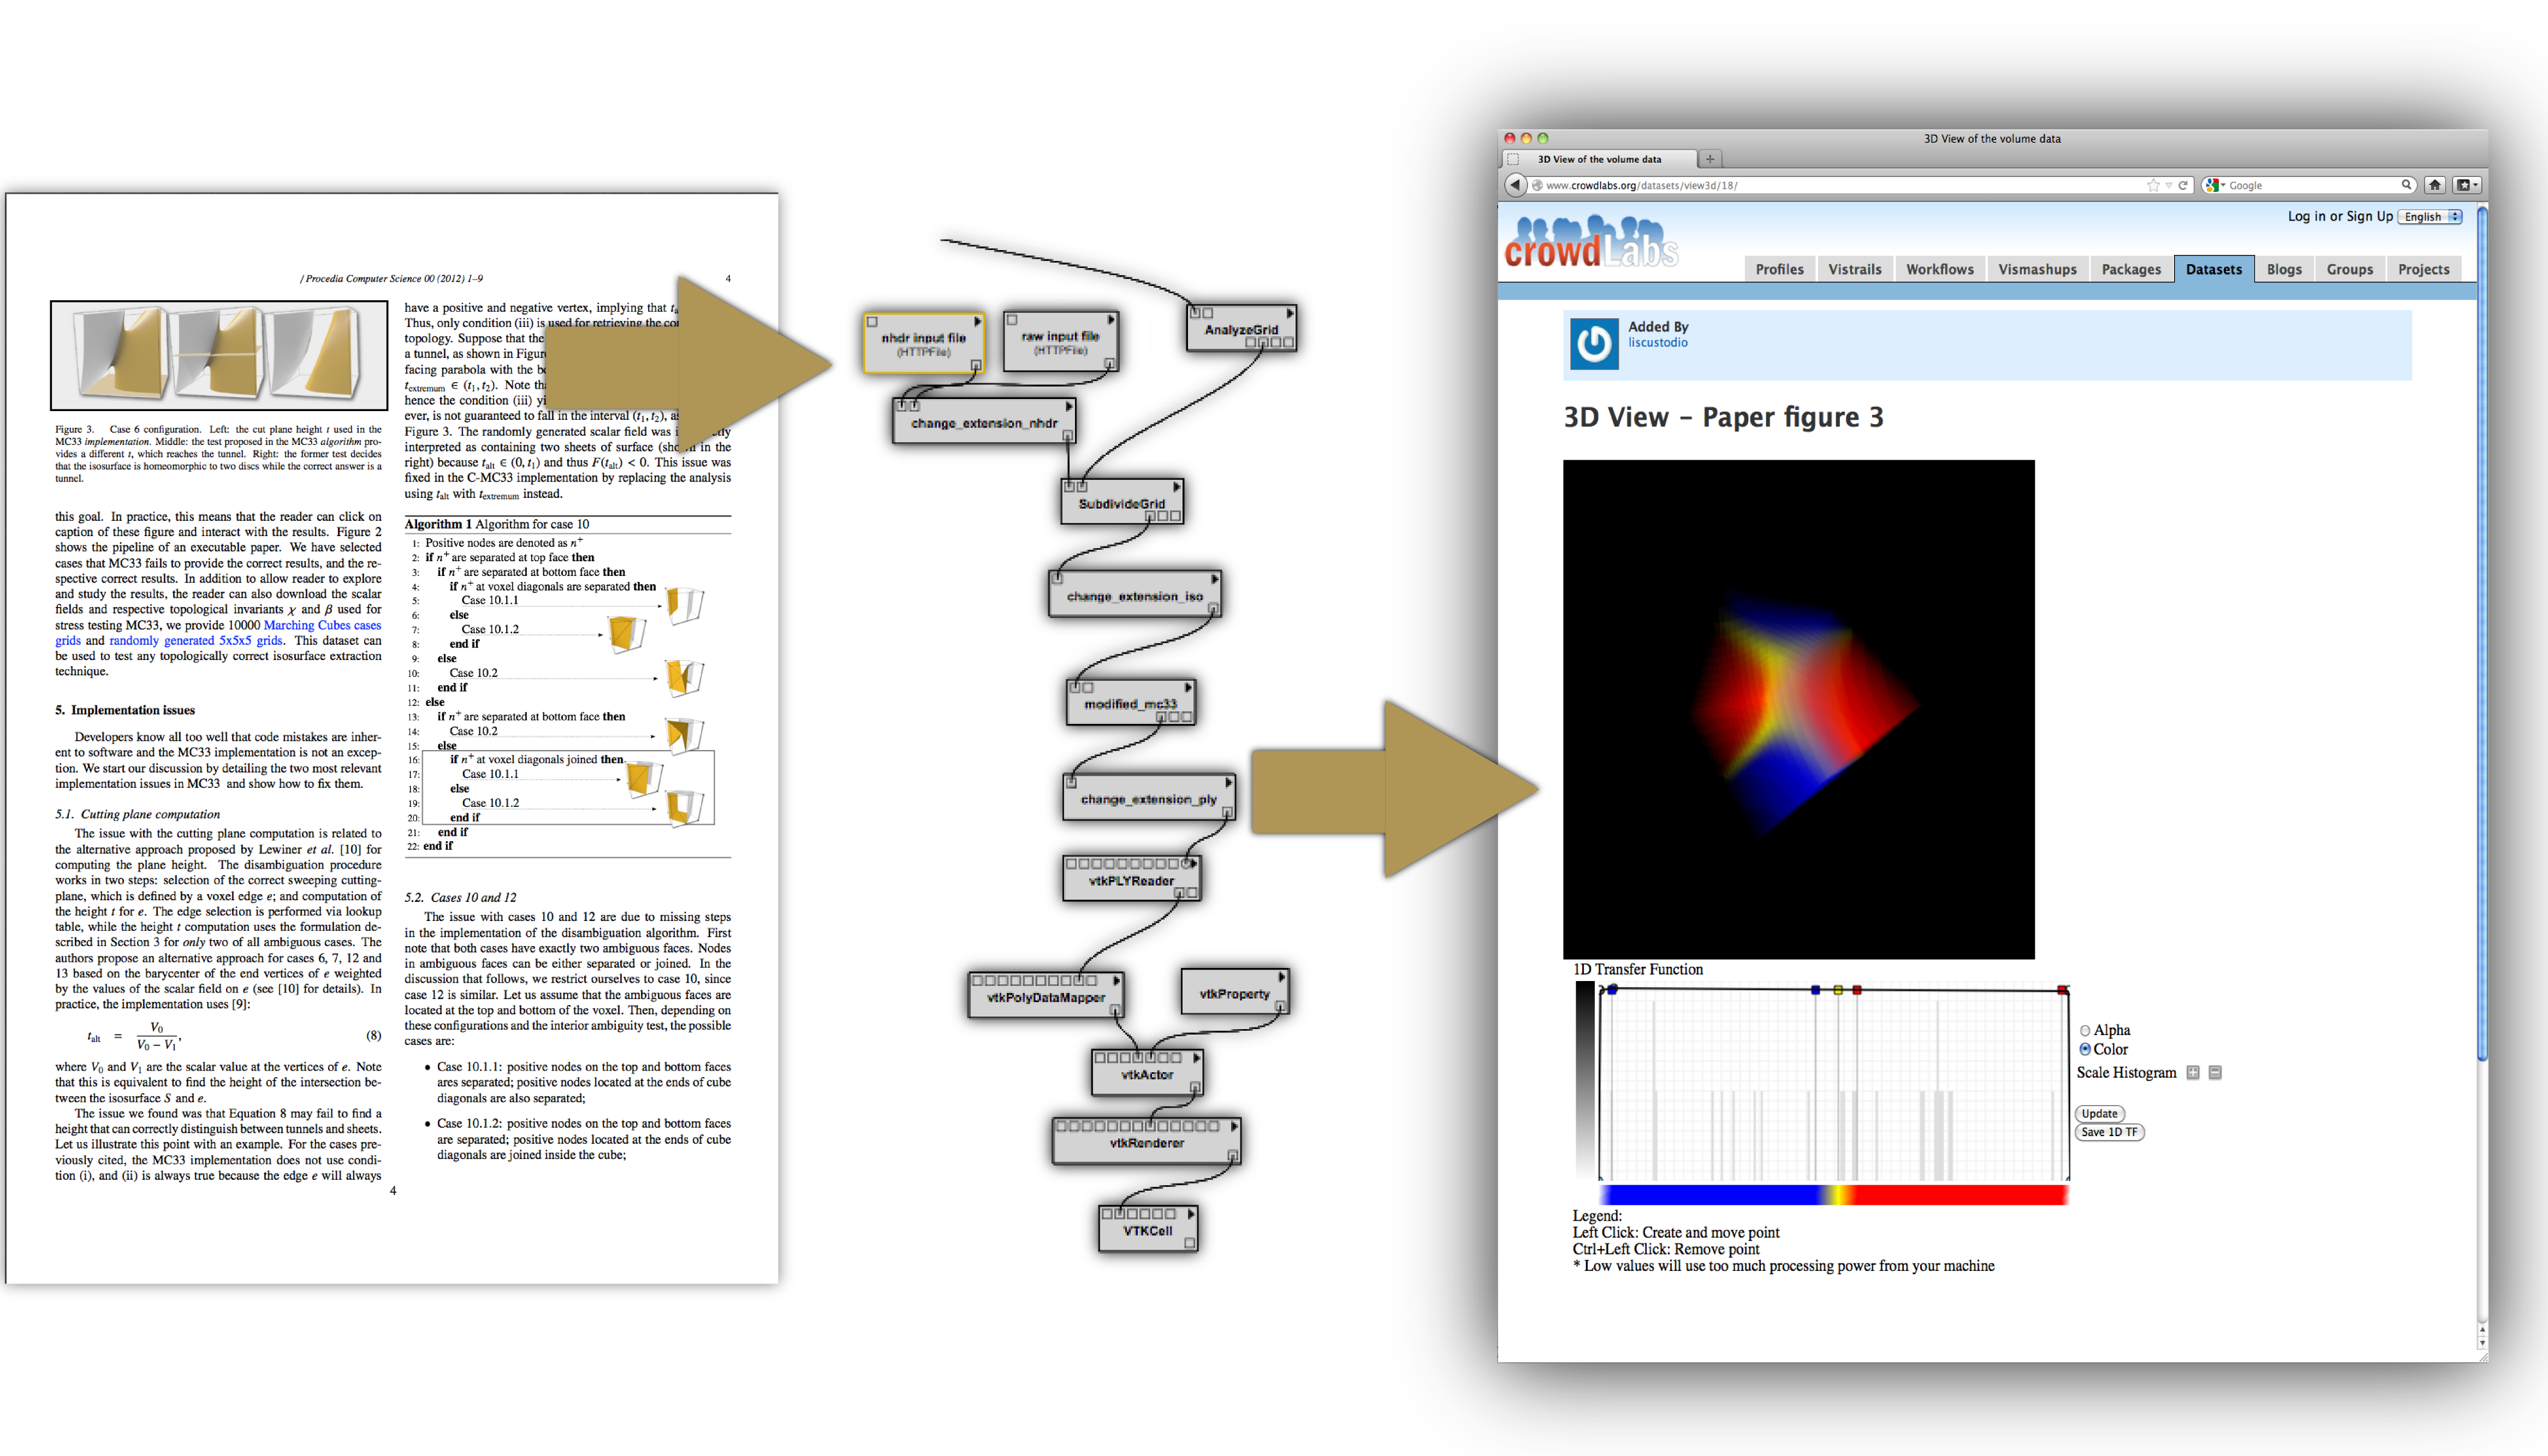
\includegraphics[width=0.7\linewidth]{chapter4/figures/executable.png}
     \caption{ \label{fig:executable}\href{http://liscustodio.github.io/C_MC33/index.html}{The executable paper pipeline. An image is made executable (left), meaning that the reader can launch a request to execute a pipeline in a remote server (middle) and interact with the result in a web browser (right) \cite{lisOnline2013}.}}
\end{figure}

As investigators in a mature field within the scientific visualization community, isosurface extraction researchers have developed ways to help other researchers and practitioners reproduce their results. Published journal articles offer a first approximation of reproducibility. Nevertheless, many details regarding implementation, source code, input data, and other types of information are often omitted. Many, but not all, published techniques make source code and input data freely available, and some are part of widely used visualization packages such as VTK~\cite{vtk}. This practice greatly increases the degree of reproducibility of the work. 
We use CrowdLabs~\cite{Tohline:2010jn} and Vistrails~\cite{Freire:2006va, Silva:2007:PVR:1300781.1302461} as a platform to achieve this goal. To explore some of the results shown in this chapter, the  reader may click on individual figure captions and interact with the results via web browser. Figure \ref{fig:executable} shows the pipeline of an executable paper. 
%
We have selected cases in which \mc{} fails and have provided the respective correct results. In addition,  to allow the reader to explore and study the results presented here, he or she can also download the scalar fields and respective topological invariants $\chi$ and $\beta$ used for stress testing \mc. We also provide 10000 \href{http://liscustodio.github.io/C_MC33/MarchingCubes_cases.zip}{\textcolor{blue}{Marching Cubes cases grids}} and \href{http://liscustodio.github.io/C_MC33/Closed_Surfaces.zip}{\textcolor{blue}{randomly generated 5x5x5 grids}} \cite{lisOnline2013}. This dataset can be used to test any topologically correct isosurface extraction technique.



\section{Issues with the \mc{}}
\label{erros_cause:chernyaev}

In this section, we discuss specific issues regarding both Chernyaev~\cite{Chernyaev95marchingcubes} and Lewiner \emph{et al.}'s~\cite{Lewiner:2003} work. Because Lewiner \emph{et al.} extends Chernyaev's work, the issues presented in the latter are also part of the former. Specifically, we detail three \emph{algorithmic} issues -- two in Chernyaev's \mc{} and one in Lewiner \emph{et al.}  --  and one \emph{implementation} issue. The solutions for the issues raised here will be presented in the next section.

This section is organized as follows. First, we explain an algorithmic problem with the \mc{} core disambiguation procedure. This issue has not been discussed in the literature to date. We then discuss a second algorithmic problem related to the triangulation table and the extraction of non-manifold meshes. Although this problem has been discussed in the literature, we discuss it here for completeness and because we provide an alternative  solution to the problem (see Section \ref{sec:solution}). Next, we show a third algorithmic problem related to the alternative approach proposed by Lewiner \emph{et al.} for computing the height plane $t$. Lastly, we show a non-trivial problem with the open-source implementation of the \mc{}. 

\subsection{Issue I -- Case 13.5}
\label{sec:problem-case-13}

Here, we show a problem with the core disambiguation procedure described in Chernyaev's work. To our knowledge, this problem has not been exposed or addressed in the literature.

Case 13 is certainly the most complex table case; all faces are ambiguous, and six subcases are possible. Four of the subcases can be discriminated by using Asymptotic Decider. The remaining cases 13.5.1 and 13.5.2 require Chernyaev's \mc{} interior ambiguity resolution method.
%
Recall that the \mc{} approach discriminates between tunnels and isolated sheets by finding a cutting-plane for which positive nodes in the cube diagonal are joined by points in the interior of the cubic cell (see Figure \ref{interior_ambiguity}). 
Cases 13.5.1 and 13.5.2 differ precisely because the positive nodes in case 13.5.2 are connected to one another by interior points, which is not true for 13.5.1 (see Figure \ref{fig:case13}).

\begin{figure}[b]
     \centering
     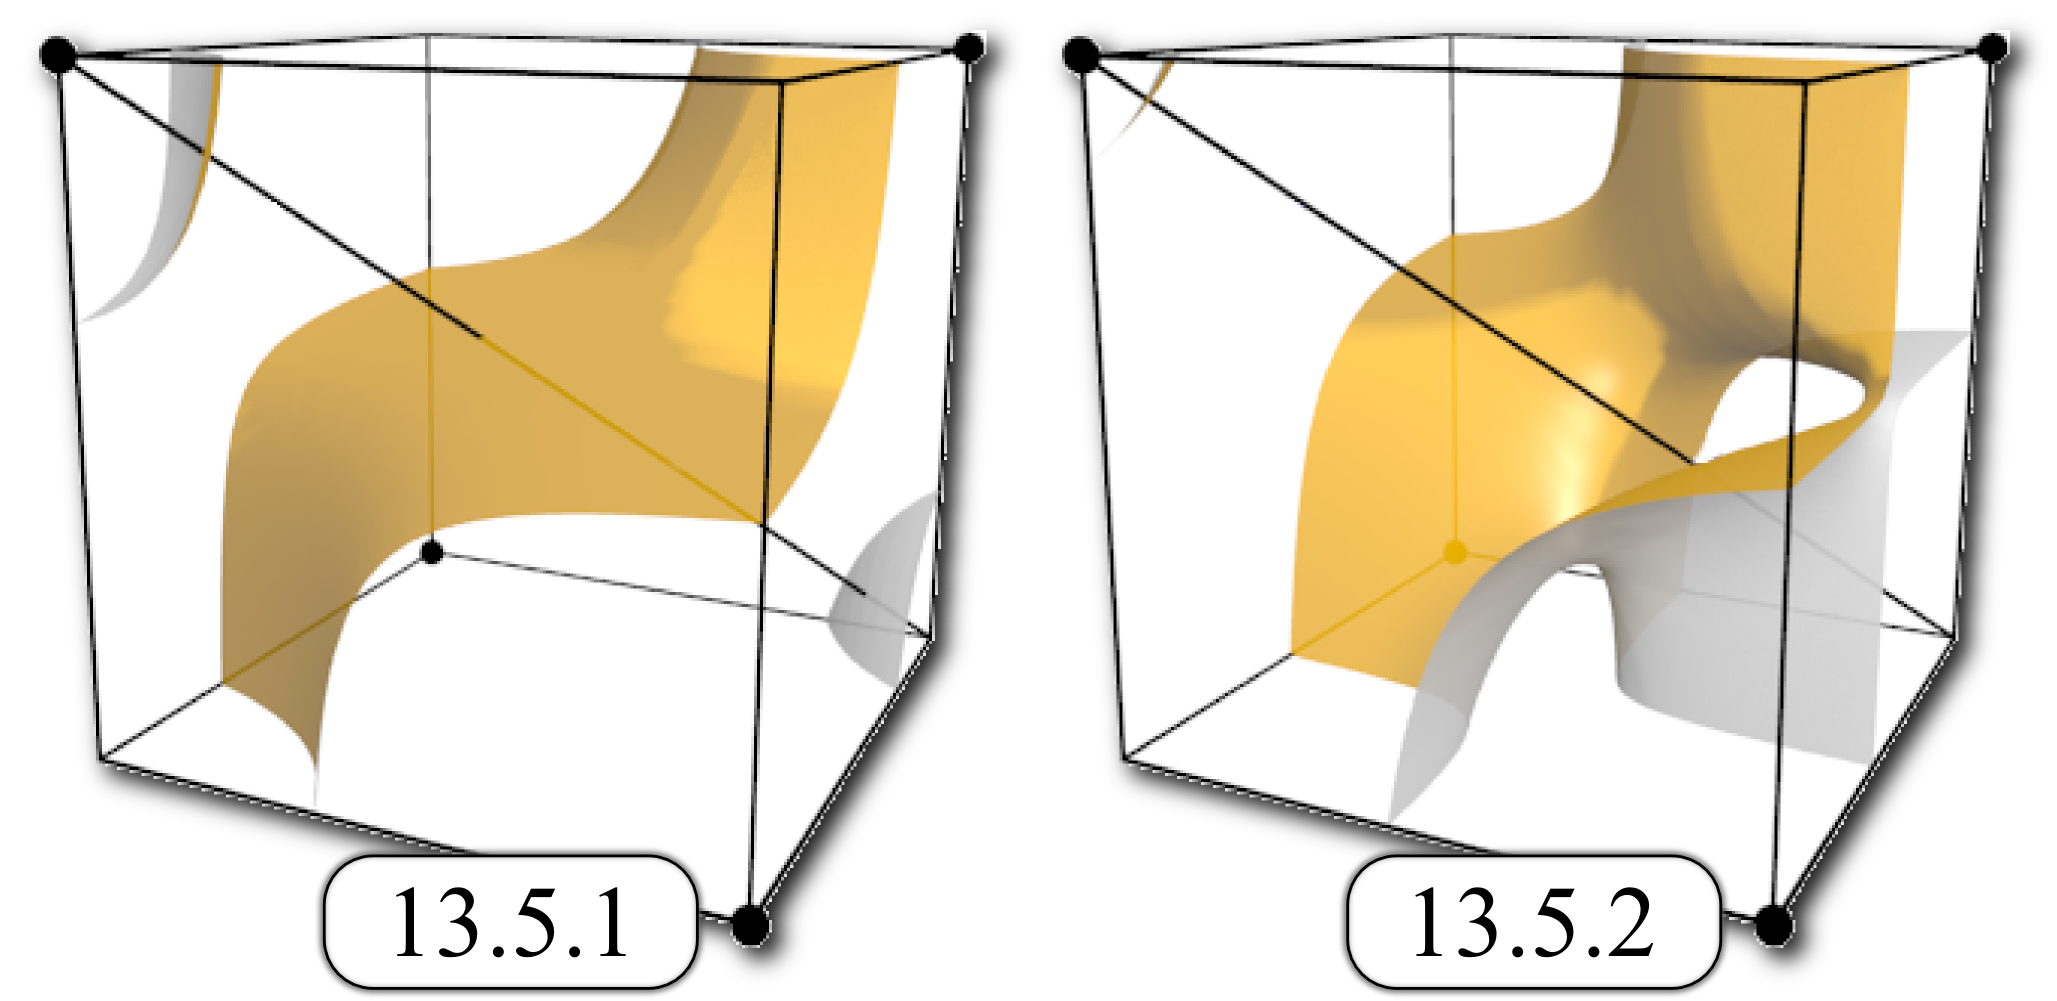
\includegraphics[width=0.6\linewidth]{chapter4/figures/case-13.png}
     \caption{Challenging cases for Chernyave's interior test: voxel diagonal has vertices with opposite signs. Case 13.5.2 needs to be oriented correctly. One of the diagonal vertices is isolated from all other vertices in the cube, while the other is faced by the tunnel. In order to determine which vertex is isolated, we apply the same tool used for disambiguation of case 13.5. For case 13.5.1, the orientation of the isosurface have no influence on the topology. }
     \label{fig:case13}
\end{figure}


\begin{figure}[b]
     \centering
     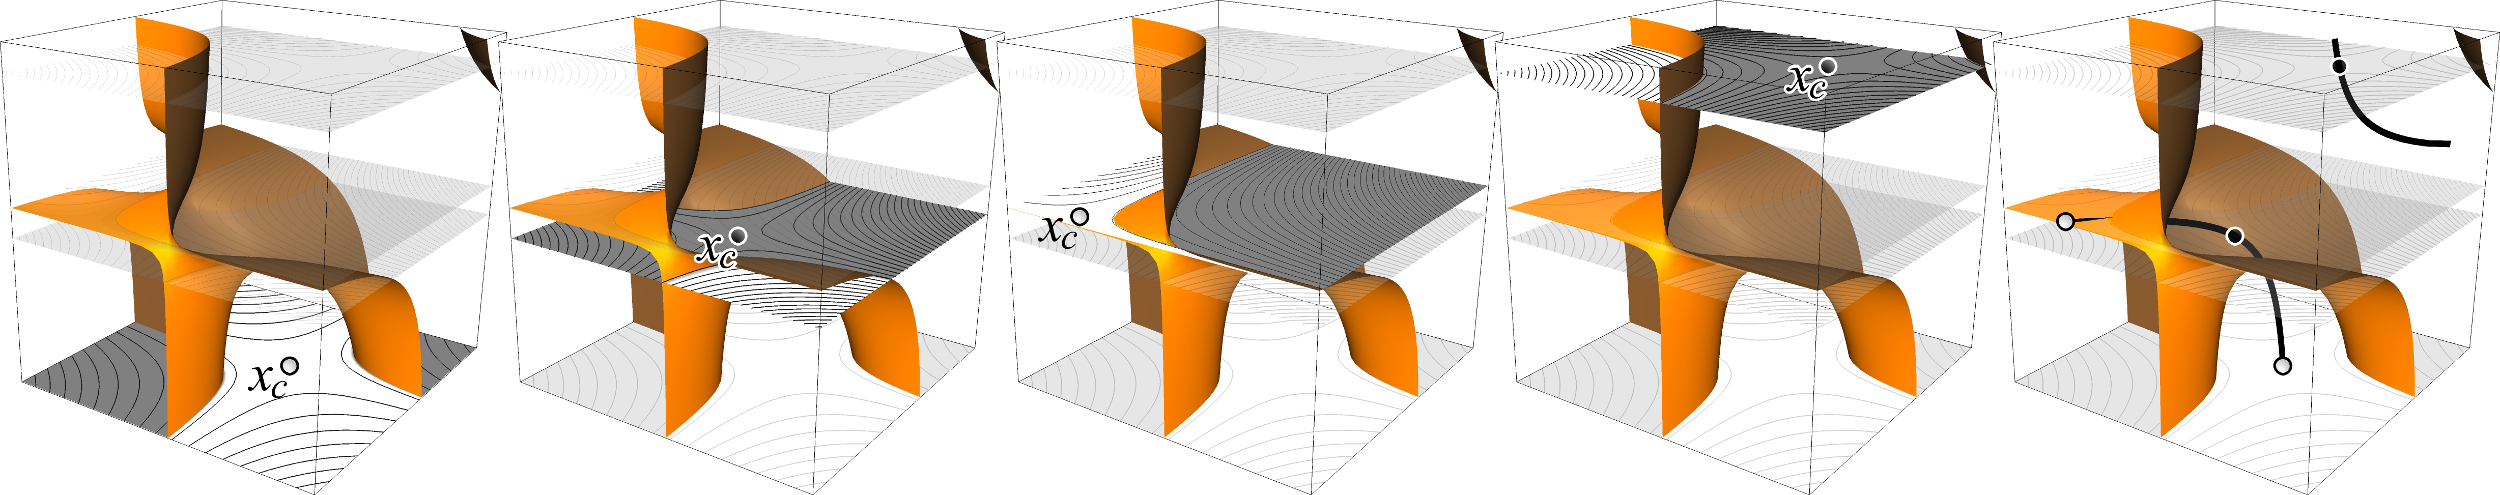
\includegraphics[width=0.99\linewidth]{chapter4/figures/case13/case13.png}
     \caption{Sign changes of the cutting-plane saddle point as a function of the height $t$. The gray area depicts $f(x) > 0$. The black (resp. white) dots are face saddles with $f(x_c) > 0$ (resp. $f(x_c) < 0$). From left to right, the four leftmost images show the sign of the face saddle points changing from negative to positive to negative and to positive again, respectively. The rightmost image shows the  hyperbolic trajectory of the face saddle position $x_c(t)$. The \mc{} algorithm fails to track the saddle point sign because it ignores the influence of the hyperbolic trajectory shown here. }
     \label{fig:case13saddlesigns}
\end{figure}

\begin{figure}[t]
     \centering
     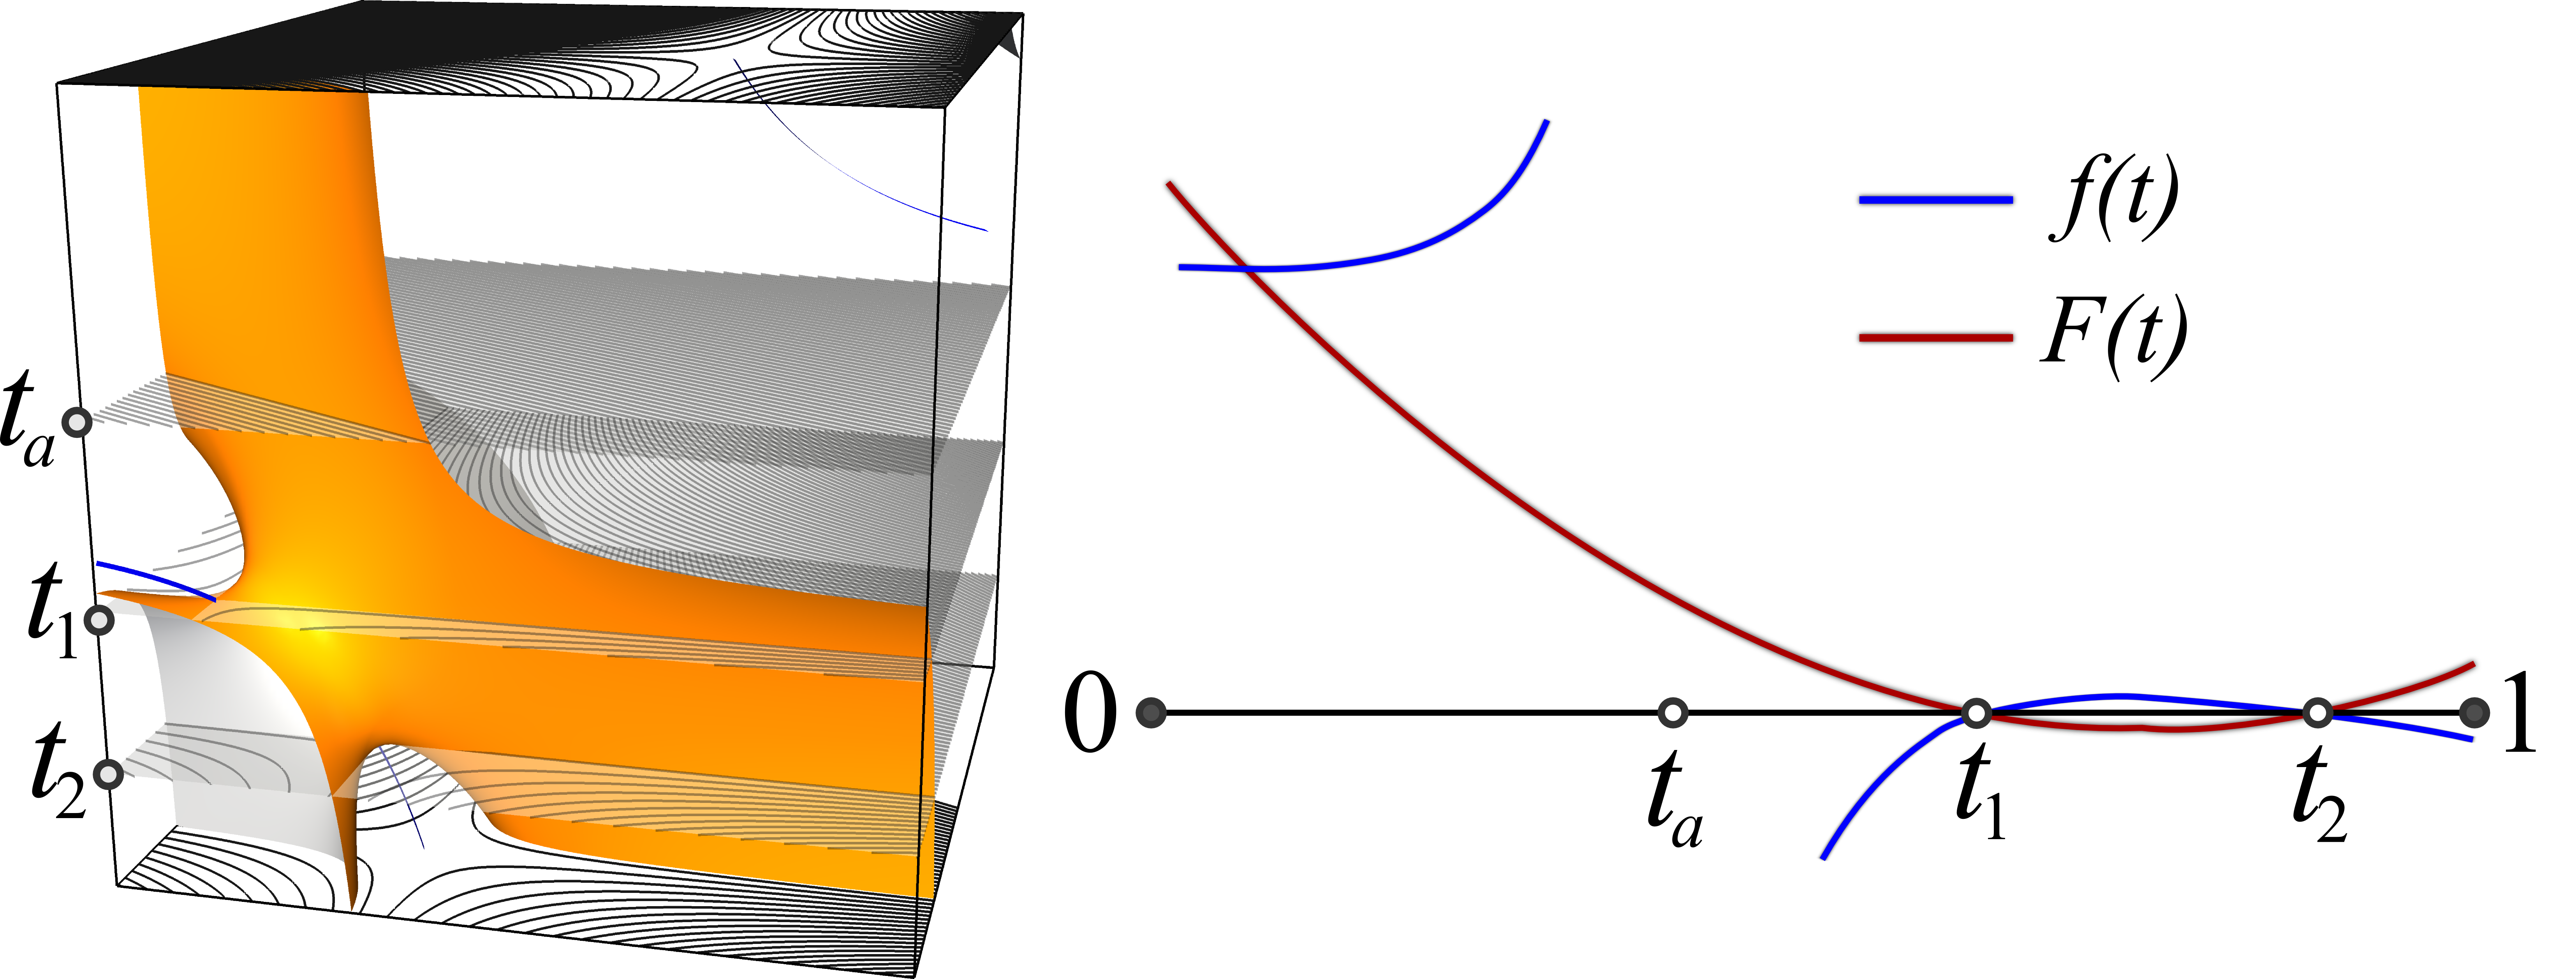
\includegraphics[width=0.7\linewidth]{chapter4/figures//graph.png}
     \caption{Counterexample to Chernyaev's core disambiguation algorithm. The \mc{} algorithm incorrectly interprets case 13.5.2 as 13.5.1. The left image shows the zero-level set for case 13.5.2 and cutting-planes at heights $t_1$, $t_2$, and $t_a$, which correspond to both roots of $F(t)$ and the asymptote of $f(x_c(t))$, respectively. The blue ribbon shows the path of the face saddle $x_c(t)$. The right image shows the changes in $f(x_c(t))$ and $F(t)$. According to the three criteria of the \mc{} algorithm described in Section \ref{sec:preliminaries},  the upward-facing red parabola defines the absence of a tunnel (condition (i)), which is incorrect. The blue curve, on the other hand, shows the correct sign change.}
     \label{fig:case13counter_example}
\end{figure}

Although it seems that the \mc{} methodology described in Section \ref{sec:preliminaries} fits naturally in this scenario, as it turns out this disambiguation procedure \emph{cannot} be applied for 13.5. 
%
Let us illustrate this point with an example. Figure \ref{fig:case13saddlesigns} shows the expected changes in the sign of the saddle point $x_c$ as a function of the height $t$. Mathematically
\begin{eqnarray}
x_c(t) & = & \left( \frac{A_t - D_t}{A_t+C_t-B_t-D_t}, \frac{A_t - B_t}{A_t+C_t-B_t-D_t} \right).
\end{eqnarray}
It follows that the face saddle value (and thus sign) is also defined as a function of $t$:
\begin{eqnarray}
f(x_c(t)) &=& \frac{A_tC_t - B_tD_t}{A_t+C_t-B_t-D_t}\\
       &=& \frac{a t^2 + b t + c}{A_t+C_t-B_t-D_t}.
\end{eqnarray}
As can be seen in Figure \ref{fig:case13saddlesigns}, from left to right, as the plane height $t$ changes, the value of the face saddle $f(x_c(t))$ changes from negative to positive to negative and to positive again. These changes occur at the roots $t_1$ and $t_2$ of $f(x_c(t))$ and the asymptote of $f(x_c(t))$, {\em i.e.}, the root $t_{a}$ of the denominator of $f$ (see left image in Figure \ref{fig:case13counter_example}). Thus, in total, three sign changes will occur. The rightmost image in Figure \ref{fig:case13saddlesigns} shows the path traced by the face saddles $x_c(t)$; as $t$ grows, there is a ``jump'' not only in the sign of $f(x_c(t))$ but also in the position of $x_c(t)$ . The change occurs precisely when the height $t$ passes through the asymptote of $f(x_c(t))$.

Nevertheless, contrary to what is expected, the polynomial $F(t)$ (Equation \eqref{eq:disambiguation}), used by Chernyaev's \mc{} algorithm for tracking the sign of the saddle point, is a second order equation in $t$ and thus can only allow for two sign changes. Therefore, the sign tracked by the \mc{} algorithm will not match the expected one at some point. Because the sign of the saddle points is embedded in all three  conditions for verifying the presence or absence of tunnels, \mc{} will eventually provide a wrong result.

The source of the problem can be tracked to Equations \ref{eq:condition1} and \ref{eq:condition2} and the assumption that the denominator of $f(x_c)$ (Equation \eqref{eq:saddle_value}) is positive. 
These assumptions can easily be verified to be true for case 4, shown in Figure \ref{interior_ambiguity}. However, for case 13, the saddle points at the top and bottom planes have opposite signs, which contradicts Equations \eqref{eq:condition1} and \eqref{eq:condition2}. In addition, the denominator $A+C-B-D$ of $f(x_c)$ changes its sign at the asymptote of $f(x_c)$, contrary to the assumption that it is always positive.
%
The consequence of incorrectly tracking sign changes is that the three rules used for resolving internal ambiguity will fail for some scalar fields. As an example, Figure \ref{fig:case13counter_example} shows a case 13.5.2 that will mistakenly be taken as case 13.5.1 because  $a > 0$ characterizes multiples surface sheets instead of a tunnel (see also \ref{app:counter-example}).
%
The problem is not only related to the misclassification of case 13.5.2 as 13.5.1. We have also devised examples in which case 13.5.1 is mistakenly taken as case 13.5.2 because the three criteria shown in Section \ref{sec:preliminaries} hold. Thus, Chernyaev's interior ambiguity test does not always yield topologically correct isosurfaces.

\subsubsection{Tunnel orientation}

\begin{figure}[b]
     \centering
     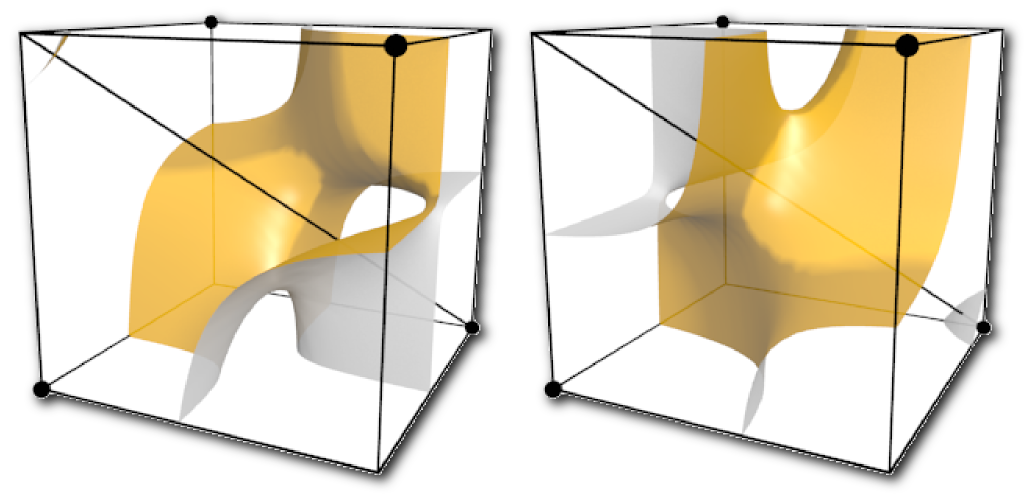
\includegraphics[width=0.6\linewidth]{chapter4/figures/tunnel.png}
     \caption{Two possible tunnel orientations for case 13.5.2. The difference between them is the location of the positive vertex.}
\end{figure}
A second minor issue regarding case 13.5.2 is the tunnel orientation of configuration 13.5.2. Once case 13.5.2 is determined, one needs to properly orient the tunnel inside the voxel. The inline figures show the two possibilities. Both vertices at the voxel diagonal are separated from all other voxel vertices at the voxel faces (note that this is not the case for other vertices). Nevertheless, either the positive or the negative vertex of the cube diagonal will connect with vertices with the same sign through the voxel's interior. This will determine which vertex is isolated and which is facing the tunnel. This problem with the tunnel orientation is not dealt with or mentioned in either Chernyaev or Lewiner \emph{et al.}'s work. Nevertheless, it was briefly mentioned in Etiene \emph{et al.} \cite{Etiene:2012:TVI:2197070.2197097}, but no solution to the problem was provided. As the authors observed, the isosurface topology changes if the tunnel orientation is incorrect; thus, it must be oriented correctly. The section \ref{sec:TunnelOrientation} provides a solution for this issue.

\subsection{Issue II -- Non-manifold surfaces}
\label{sec:non-manifold-surfaces}

\begin{figure}[b]
     \centering
     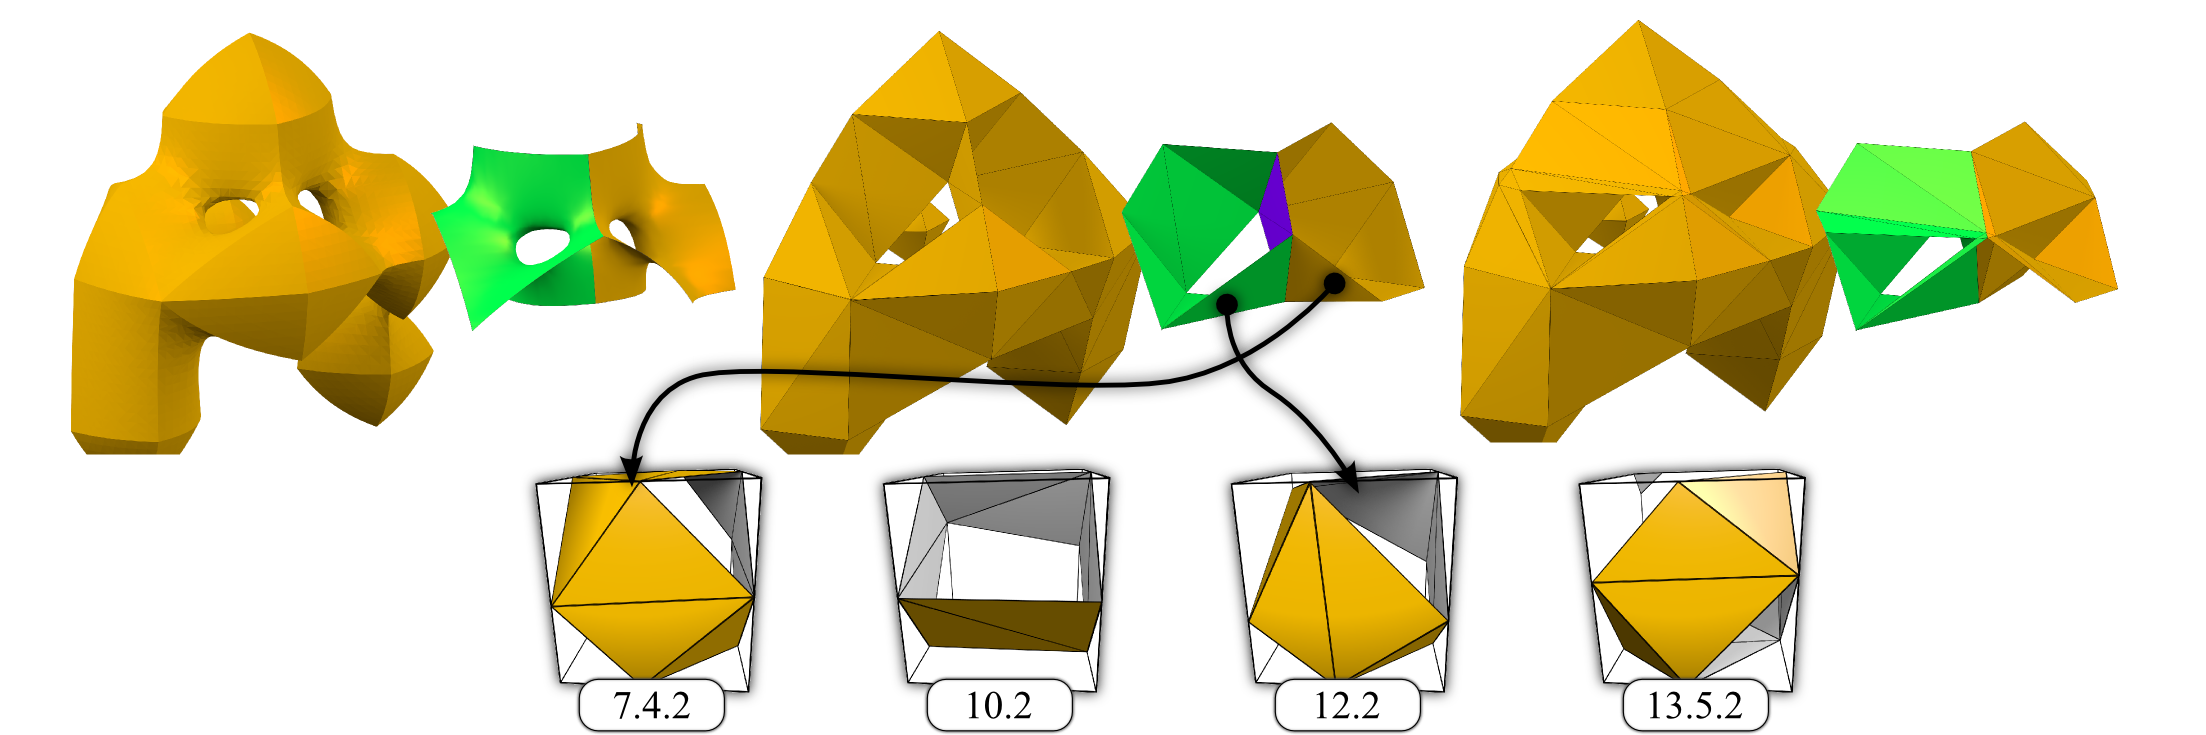
\includegraphics[width=0.9\linewidth]{chapter4/figures/non_manifold.png}
     \caption{\href{http://liscustodio.github.io/C_MC33/figure8.html}{Top: Problem with Chernyaev's triangulation table. The figure shows the  zero level-set of a $5\times5\times5$ randomly generated piecewise-trilinear scalar field $G$ (left) and two meshes extracted using the \mc{} (center) and \cmc{} (right) algorithms. The isolated voxel patches, shown in green and yellow, represent the two voxels at the center of $G$. The face shared by two consecutive tunnels, shown in purple, generates non-manifold edges. After one subdivision at the critical point of this case, the problem no longer occurs, and a valid manifold surface is obtained (right). Bottom: Triangulation for tunnels used by Lewiner \emph{et al.}~\cite{Lewiner:2003}. Each has a face that is coplanar to the voxel faces, which may lead to non-manifold surfaces.} \cite{lisOnline2013}}
  \label{fig:non_manifold}
\end{figure}

The second algorithmic issue is related to the triangulation table used to build triangulated surfaces.
%
The choice of the correct MC configuration is only part of the process of building an algorithm that preserves the topology of the piecewise-trilinear field. The voxel triangulation table is, in fact, the determinant of the final mesh topology.  Chernyaev's original triangulation table contains cases that lead to topologically inconsistent non-manifold meshes in scenarios such as the one shown in Figure \ref{fig:non_manifold}. 
%
This problem occurs because the \mc{} triangulation table allows faces that are coplanar with the grid voxel faces. Hence, when neighbor voxels have ``tunnels'' in their interiors, and share an ambiguous, coplanar face, the end result will be non-manifold edges, as shown in Figure \ref{fig:non_manifold}.
%
Because this is an issue with the triangulation table, any topologically correct algorithm whose table is based on Chernyaev's triangulation table will build non-manifold surfaces whether or not the algorithm can correctly distinguish the voxel cases.

This problem with Chernyaev's work was pointed out by Lopes and Brodlie \cite{lopes:tvcg:2003} (following earlier work by Van Gelder and Wilhelms \cite{Gelder94topologicalconsiderations}) and is one of the motivations of Lopes and Brodlie's work on topologically correct and geometrically accurate isosurface extraction algorithm \cite{lopes:tvcg:2003}. Lopes and Brodlie aimed at improving the geometry quality of the trilinear surface patches and consequently solving the topology problem. They achieve this goal by adding points to the voxel faces as well as to the voxel interior. These extra points are placed on the trilinear patch which increases geometry accuracy. They are classified into three different classes and used for extending the contour of the trilinear patch with the voxel faces. The implementation of this technique becomes intricate and error-prone due to the additional steps required for voxel triangulation. 


\subsection{Issue III -- Cutting-plane computation}

The third algorithmic issue is related to an \mc{} improvement proposed by Lewiner \emph{et al.}~\cite{Lewiner:2003} for computing the plane height.  
The problem is that Equation \eqref{eq:alternative} may fail to find an appropriate height  that can correctly distinguish between tunnels and surface sheets. Let us illustrate this point with an example. For the cases previously cited, two of the conditions in the Chernyaev interior test described in Section \ref{sec:preliminaries} are not used. The \mc{} implementation does not use condition (i), and (ii) is always true because the edge $e$ will always have a positive and a negative vertex, implying that $t_{\mathrm{alt}} \in (0,1)$. Thus, only condition (iii) is used in retrieving the correct voxel topology. Suppose that the scalar field in a given voxel defines a tunnel, as shown in the left image in Figure \ref{interior_test}. In this case, to retrieve the correct topology, $F(t)$ should be a downward-facing parabola with both roots $t_1, t_2 \in (0,1)$, $t_1 < t_2$, and $t_\mathrm{max} \in (t_1,t_2)$. In this case, $F(t) > 0$ only for $t \in (t_1, t_2)$; hence, $F(t_{\mathrm{max}}) > 0$, and a tunnel is retrieved according to condition (iii). The problem with the alternative approach is that, as shown in Figure \ref{interior_test}, the solution to Equation \eqref{eq:alternative} is not guaranteed to fall within  the $(t_1,t_2)$ interval, which implies that the scalar field may be incorrectly interpreted as containing two sheets of surface (shown on the right). In other words, because $t_{\mathrm{alt}} \in (0,t_1)$ and $F(t_{\mathrm{alt}}) < 0$, condition (iii) verifies the absence of a tunnel. 

\begin{figure}[b]
     \centering
    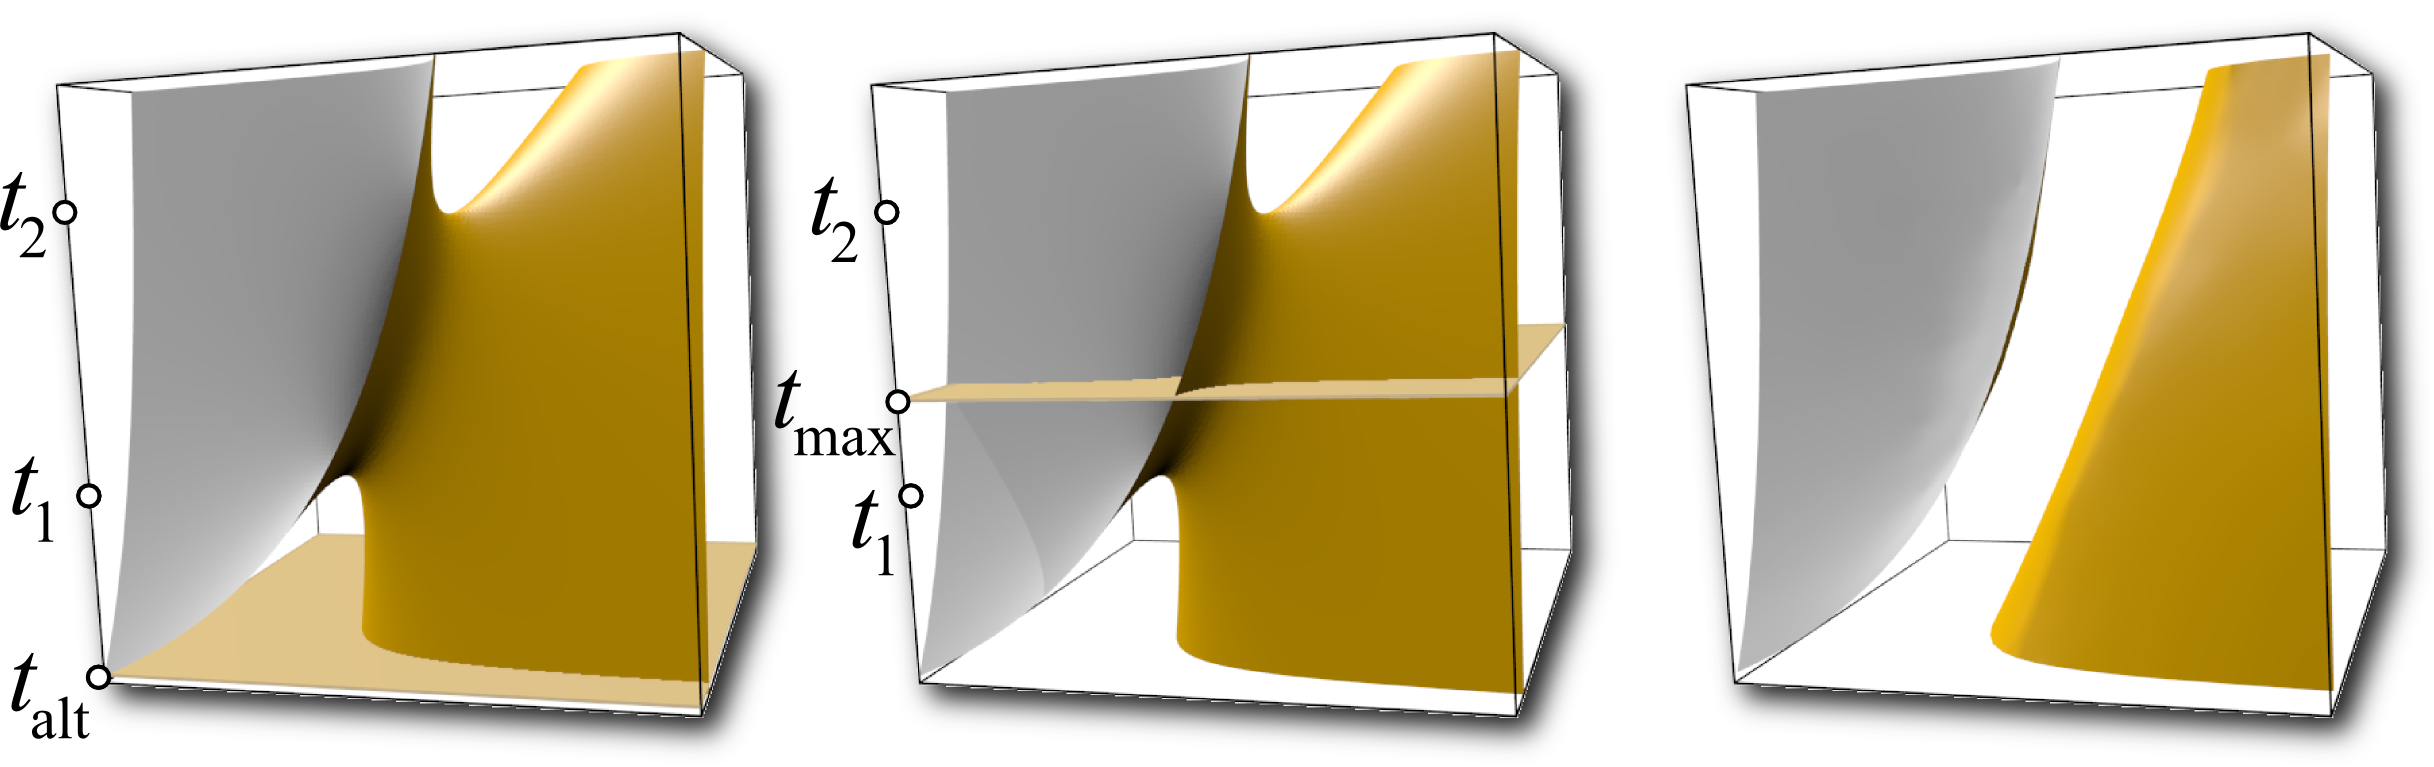
\includegraphics[width=0.95\linewidth]{chapter4/figures/height-plane-problem.png}
     \caption{\href{http://liscustodio.github.io/C_MC33/figure9.html}{\label{interior_test}Case 6 configuration.
     Left: the cut plane height $t = t_{\mathrm{alt}} > 0$ used in the \mc{} \emph{implementation}. Middle: the test proposed in the \mc{} \emph{algorithm} provides a different $t = t_{\mathrm{max}}> 0$, which reaches the tunnel. Right: the former test decides that the isosurface is homeomorphic to two discs whereas the correct answer is a tunnel.} \cite{lisOnline2013}}
\end{figure}

\subsection{Issue IV -- Case 10}
\label{erros_cause:lewiner}

The last issue described in this work is related to the implementation of \mc{}.
Developers know all too well that code mistakes are inherent to software and the \mc{} implementation is not an exception.

Due to a missing step in the implementation of the disambiguation algorithm, \mc{} fails to correctly resolve the ambiguity in cases 10 and 12. Note that both cases have exactly two ambiguous faces and the nodes in ambiguous faces can be either separated or joined. In the discussion that follows, we restrict ourselves to case 10; case 12 is similar. 

Let us assume that the ambiguous faces are located at the top and bottom of the voxel. Then, following the algorithm proposed by Chernyaev \cite{Chernyaev95marchingcubes}, depending on the sign of the face saddles and the interior ambiguity test, one can identify the correct case (see also Algorithm \ref{chernyaev_case10}):
\begin{itemize}
\item Case 10.1.1: the positive nodes on both faces are separated, and the positive nodes at cube diagonals are also separated;
\item Case 10.1.2: the positive nodes on both faces are separated, and the positive nodes at the cube diagonals are not;
\item Case 10.2: the positive nodes are separated on the top and connected on the bottom face.
\end{itemize}

The cases shown above assume that the positives nodes at the top face are separated. But a similar reasoning must be applied to cases in which the positives nodes at the top faces are joined. In the Lewiner \emph{et al.}'s implementation the possibility that the positive nodes at the top faces are joined is missing. 

\section{Solutions}
\label{sec:solution}
 
We present solutions for the four issues raised in the previous section. 
 
\subsection{Issue I -- Case 13.5}

The disambiguation of case 13.5 has been approached in different ways for different frameworks for isosurface extraction.  For example, Nielson \cite{Nielson03onmarching} presents an algorithm that is  concerned with connectivity along edges, faces and the voxel interior. The author presents a detailed description of the behavior of the trilinear interpolant inside the cubic grid and uses these descriptions to solve the ambiguity problem in the interior. Lopes and Brodlie \cite{lopes:tvcg:2003}, on the other hand, use critical points in order to resolve some ambiguities. In this case, the sign of the critical point determines the correct configuration.
%
Unfortunately, the above solutions do not seamlessly integrate with the \mc{} algorithm. The core idea for solving interior ambiguity, namely, that tunnels can be detected by a sweeping plane through the voxel, is absent in both approaches. This motivated us to devise an alternative solution that we feel follows the idea presented in the original algorithm.

We solve this problem by proposing a new interior test that uses the fact that case 13.5.2 requires both \emph{roots} $t_1$ and $t_2$ of $f(x_c(t))$ and the associated saddle points to be inside the voxel. 
%
First, recall that $x_c(t)$ tracks the path of the face saddle inside the voxel as a function of height plane at height $t$, and $f(x_c(t))$ tracks the value (and thus the sign) of that saddle. Both functions are illustrated in the rightmost image in Figure \ref{fig:case13saddlesigns}, in which the black hyperbolic curves represent the path of $x_c(t)$ and the color of the circles represents the sign of the face saddle at a given point (white and black circles are points with negative and positive values, respectively).
%
For case 13.5.2, the path traced by the curve $x_c(t)$ must intersect the isosurface tunnel twice, once at each of the roots $t_1$ and $t_2$ of $f(x_c(t))$. 
%
This implies that both saddle points $x_c(t_1)$ and $x_c(t_2)$ must lie inside the voxel. This is not the case for 13.5.1 because the face saddle can cross the middle sheet at most once. Therefore, it suffices to verify that both roots of $f(x_c(t))$ and its saddle points are inside the voxel. Algorithm \ref{alg:new_case-13} illustrates our solution. Our algorithm is very simple, and does not require the computation of the critical points of the trilinear interpolant, or a detailed description of its behavior inside a voxel. Our algorithm uses the ideas proposed by Chernyaev in order to fix an algorithmic problem in his work.
%
We have implemented and tested this solution on \cmc{} using over 10000 randomly generated instances of case 13.5.

\begin{algorithm}
\begin{codebox}
\Procname{\proc{Case 13.5}($a, b, c$)}
\zi $\rhd$ Let $t_1$ and $t_2$ be the roots of $a t^2 + b t + c$ (Equation \eqref{eq:disambiguation})
\li \If {$t_1, t_2 \in (0,1)$ and $x_c(t_1), x_c(t_2) \in (0,1)^2$} 
\li	\Then \Return Case 13.5.2
\li	 \Else \Return  Case 13.5.1
\End
\end{codebox}
\caption{\label{alg:new_case-13}A simple disambiguation procedure for Case 13.5}
\end{algorithm}

\subsubsection{Issue II -- Tunnel orientation}
\label{sec:TunnelOrientation}

\begin{figure}[b]
     \centering
     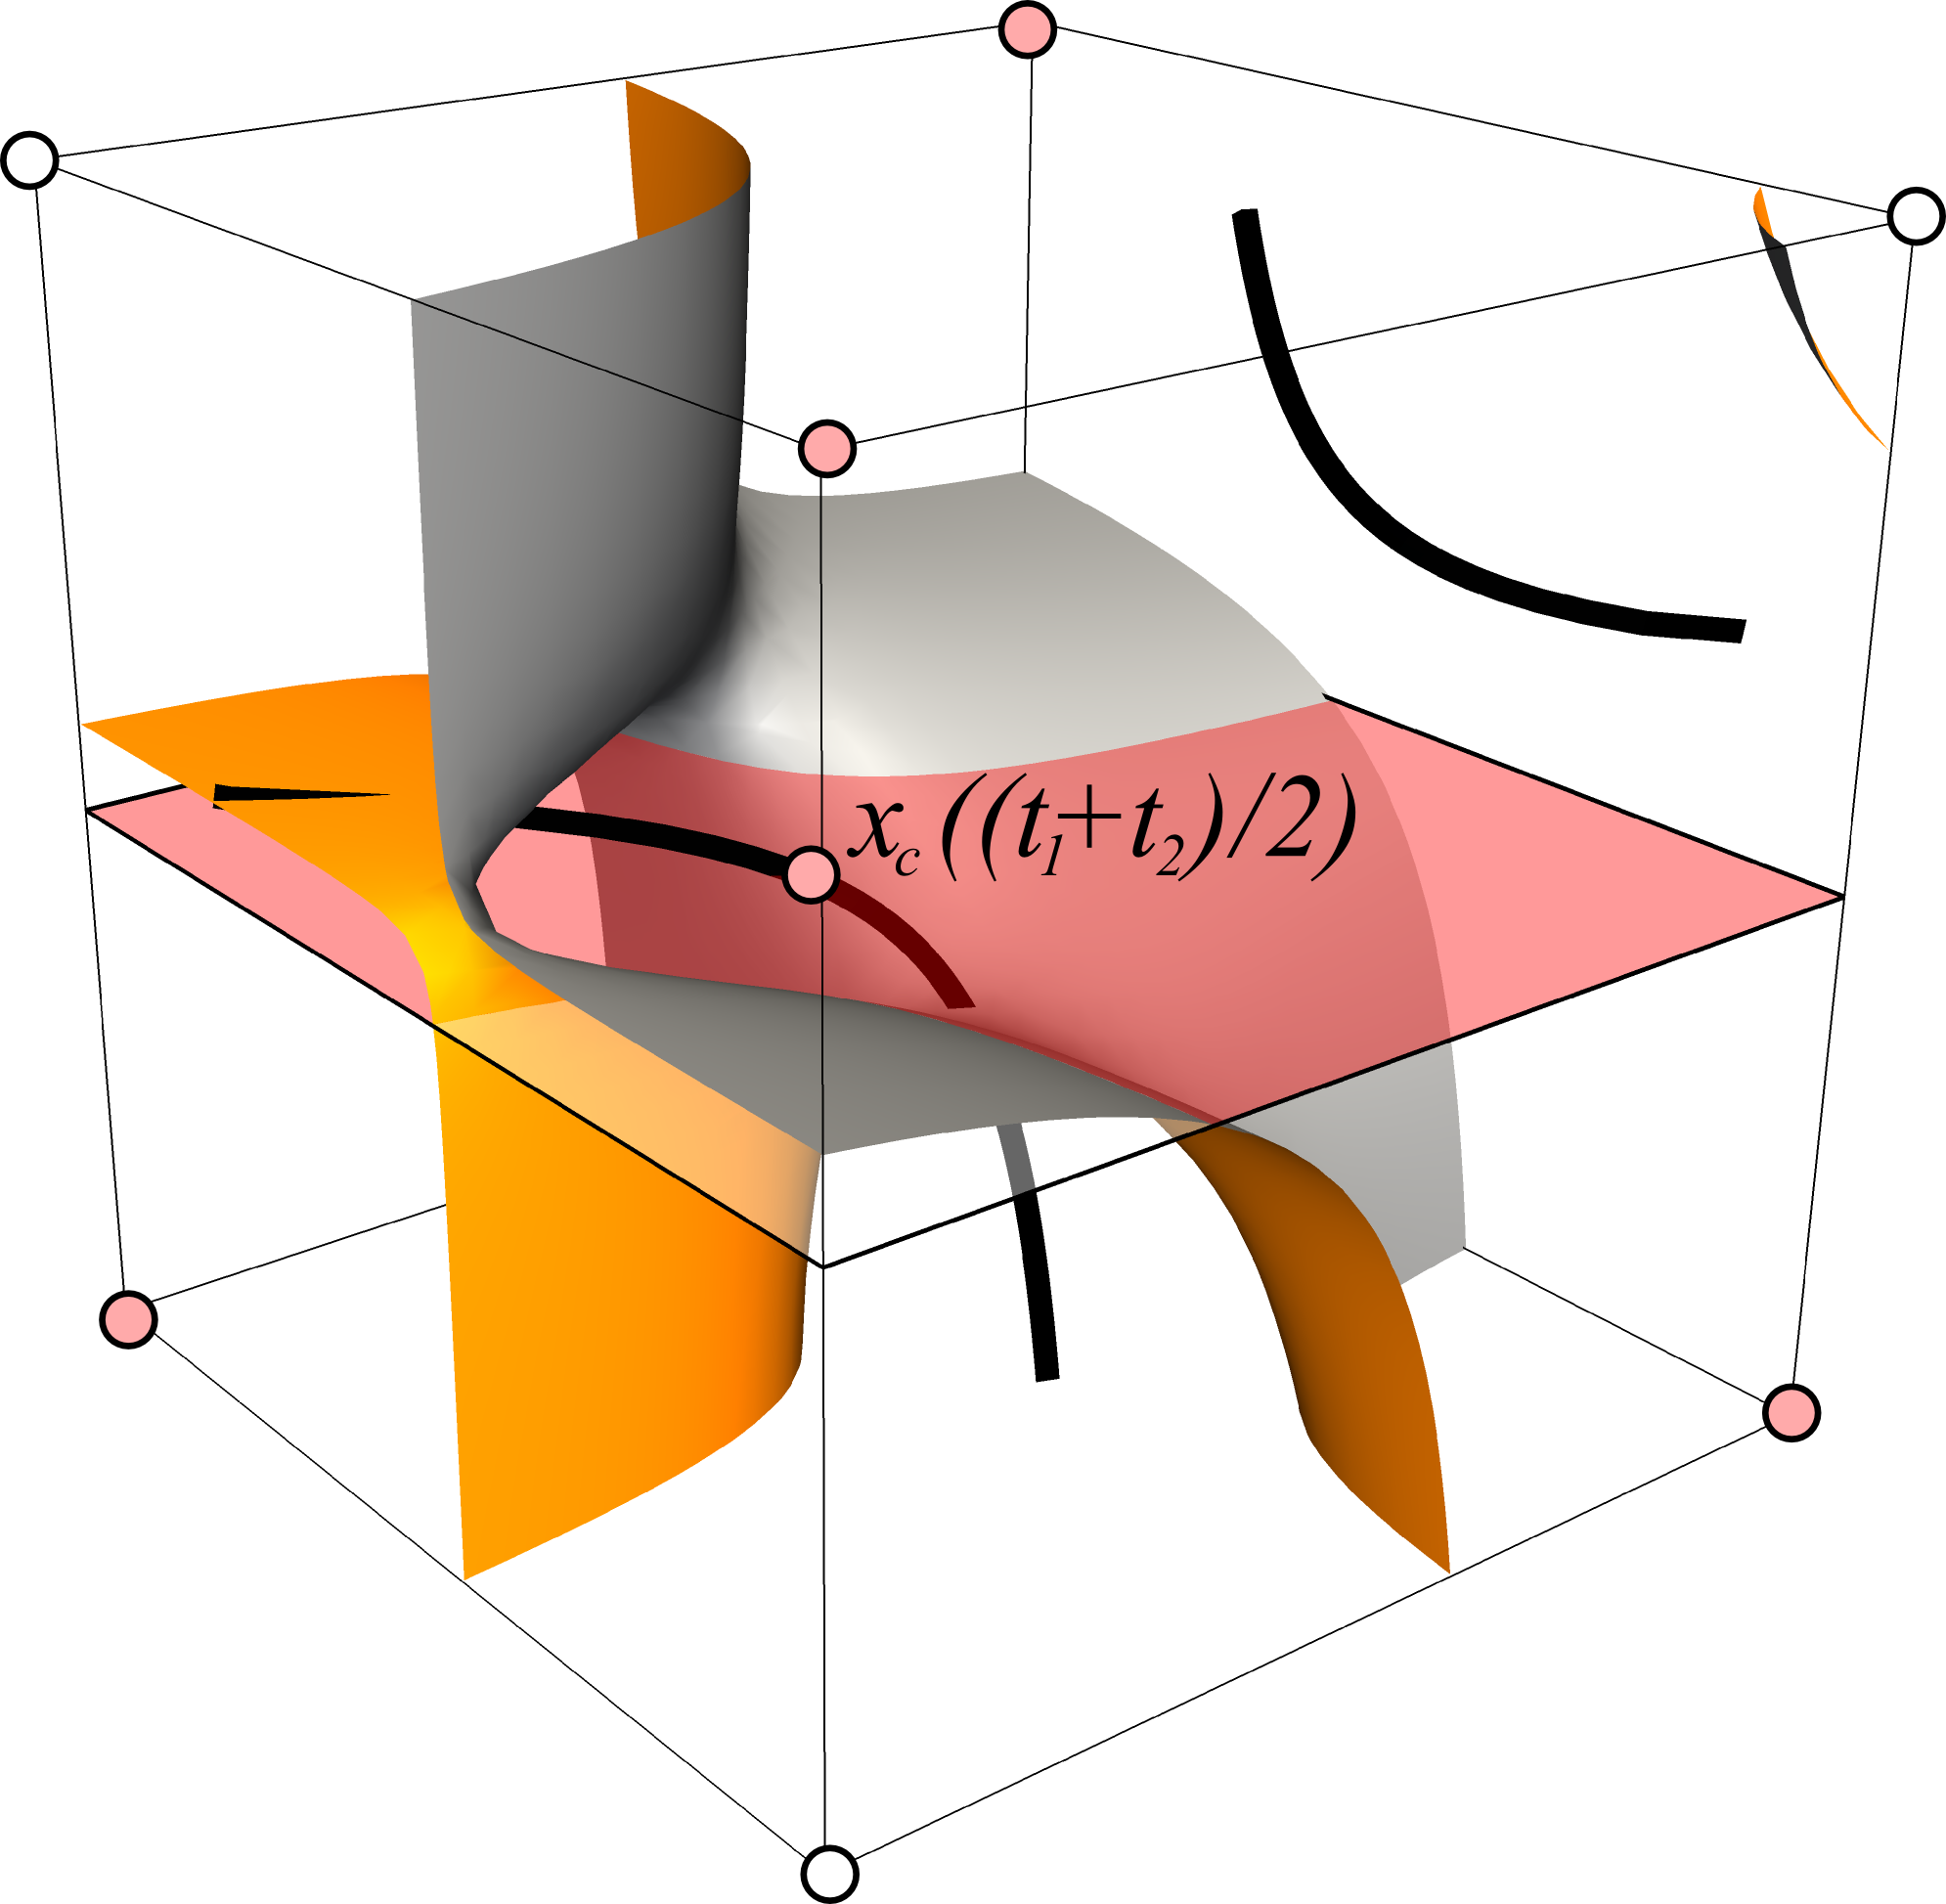
\includegraphics[width=0.5\linewidth]{chapter4/figures/case13/solution.png}
     \caption{Solution to the orientation problem. The black dots represent regions with positive scalar values.The cutting-plane location is at $(t_1 + t_2) / 2$. The sign of $f((t_1+t_2)/2)$ determines the tunnel orientation. }
     \label{fig:solution-case13}
\end{figure}

To find the correct tunnel orientation one can use the sign of any point between the roots $t_1$ and $t_2$. This is because any point in this range must have the same sign as the critical points of the trilinear interpolant for case 13.5.2. This can be seen in the black path shown in the rightmost image in Figure \ref{fig:case13saddlesigns} and from the graph in Figure \ref{fig:case13counter_example}. All points between roots $t_1$ and $t_2$ will have the same sign, which is the sign of the ``interior'' of the tunnel. Thus, we compare the sign of $f((t_1+t_2)/2)$ with the sign of both vertices of the voxel diagonal which is inside the tunnel. The tunnel will face the vertex with the same sign as $f((t_1+t_2)/2)$, whereas the other vertex must be isolated from all cube vertices. Figure \ref{fig:solution-case13} illustrates this scenario. Note that Lopes and Brodlie  \cite{lopes:tvcg:2003} used the sign of the critical points of the trilinear interpolant to retrieve the correct tunnel orientation. We provide a different solution that fits nicely with Chernyaev's framework.


\subsection{Issue II -- Non-manifold surfaces}

A possible solution to this problem involves post-pro\-cessing the mesh to remove non-manifold features. Although  many works in the literature proposed methods for fixing meshes (see \cite{springerlink:10.1007/s11390-009-9206-7} for an excellent survey), these are mainly focused on retrieving a valid manifold mesh. Topologically correct algorithms, on the other hand, require that the topology of the trilinear interpolant  be preserved. In addition, mesh repairing techniques may mask implementation issues by fixing them, which complicates the verification process. 

We use an alternative approach that does not require any changes in the \mc{} triangulation table. An interesting fact is that this problem has a low probability of being generated at random and an even lower probability of occurring in real-world datasets. For example, as shown in Figure \ref{fig:non-manifold-real-data} for the Skull dataset this problem appeared six times in total for 50 distinct isosurfaces. In our tests, it occurred only once in 10000 randomly generated $5\times5\times5$ scalar fields. Thus, instead of implementing the approach of Lopes and Brodlie's, we adopt a different solution that takes advantage of the fact that this is a rare event.

Non-manifold surfaces are created when two adjacent voxels that share an ambiguous face have tunnels in the voxel interior. By splitting both voxels at the critical point of that face, the face ambiguity is  eliminated \cite{10.1109/TVCG.2009.10}.
To simplify the algorithm, we split not only the voxels sharing the ambiguous face but all faces in the volume slice that contains that face (see Figure \ref{fig:grid-refinement}). 
%
\begin{figure}[b]
     \centering
	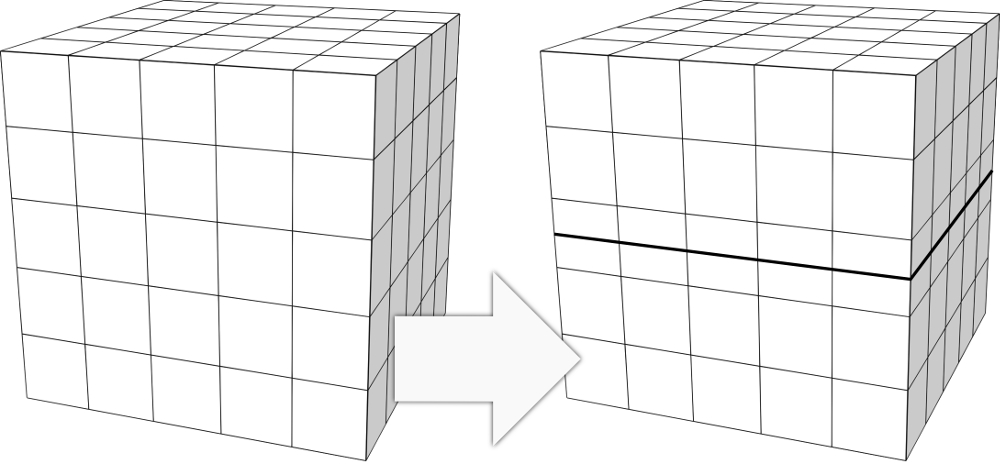
\includegraphics[width=0.5\linewidth]{chapter4/figures/grid.png}
	\caption{\label{fig:grid-refinement}Grid refinement. The slice of voxels containing the offending configuration is splitted into two slices.}
\end{figure}
%
Assuming an input of size $n \times n \times n$, each subdivision will add $n^2$ voxels to the grid.  Assuming that $k$ subdivisions are required, $k n^2$ voxels will be added. In practice $k = O(1)$, and thus $k n^2 = O(1 )O(n^2) = O(n^2)$. This implies that the asymptotic size of the dataset does not change. This subdivision adds the degree of freedom necessary to eliminate the problem, making this implementation of the Marching Cubes 33 topologically correct (see Figure \ref{fig:non_manifold}). 

\begin{figure}[b]
     \centering
     \includegraphics[width=0.9\linewidth]{chapter4/figures/cc_aneurism.png}
     \caption{\href{http://liscustodio.github.io/C_MC33/figure12.html}{Aneurysm dataset. From left to right, the displayed isosurfaces were extracted using VTK, \mc, and \cmc, respectively. We show the main brain artery component in yellow and the extra connected components in purple. From the images shown, it is clear that the purple components should be part of the main branch. Nevertheless, due to the implicit disambiguation in VTK and the issues in \mc, the final isosurface contains multiple components (left and middle figures). The isosurface generated using \cmc{} is shown on the right. } \cite{lisOnline2013}}
     \label{fig:cc_aneurism}
\end{figure}

\subsection{Issue III -- Cutting-plane computation}

Because this is a problem with the alternative method used in Lewiner \emph{et al.}, the issue can be avoided by replacing the use of $t_{\mathrm{alt}}$ with use of the originally proposed $t_{\mathrm{max}}$.

\subsection{Issue IV -- Case 10}

Algorithm \ref{chernyaev_case10} illustrates the required steps for disambiguation on case 10. We fixed the \mc{} implementation by adding the lines 16-20, which in the original implementation were replaced by the result \textit{case 10.1.1}. 

%\begin{algorithm}
%\begin{codebox}
%\Procname{\proc{Case 10}($n^+$)}
%\zi $\rhd$ Let $n^+$ be positive nodes 
%\li \If $n^+$ are separated at top faces 
%\li	\Then \If $n^+$ are separated at bottom face  
%\li		\Then  \If $n^+$  at voxel diagonals are separated 
%\li			\Then 
%\li				\Return Case 13.5.1
%\li			\Else 
%\li				\Return Case 10.1.2
%			\End
%\li		\Else 
%\li			\Return Case 10.2
%		\End
%\li	\Else 
%\li		\If $n^+$ are separated at bottom face 
%\li			\Then 
%\li				\Return case 10.2 
%\li			\Else 
%\li				\If $n^+$ at voxel diagonals are joined 
%\li					\Then 
%\li						\Return Case 10.1.1
%\li					\Else 
%\li						\Return Case 10.1.2
%					\End
%			\End
%	\End
%\end{codebox}
%\caption{\href{http://dl.dropbox.com/u/8414964/C-MC33/webpage/alg2.html}{Algorithm for case 10}}
%\end{algorithm}


\begin{algorithm}
\caption{\href{http://liscustodio.github.io/C_MC33/alg2.html}{Algorithm for case 10} \cite{lisOnline2013}}
\label{chernyaev_case10}
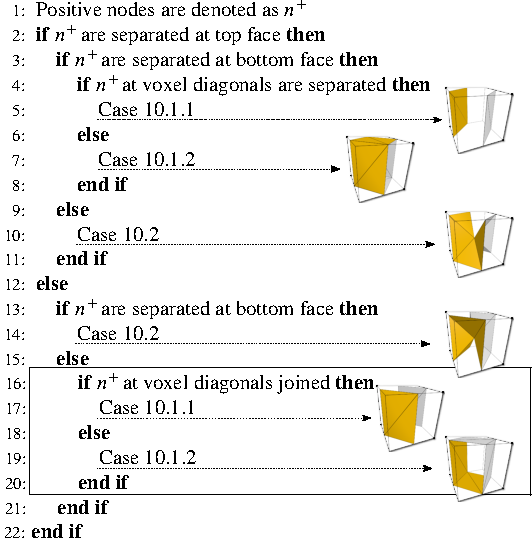
\includegraphics[width=0.7\linewidth]{chapter4/figures/algorithm.pdf}
\end{algorithm}


\section{Experiments with real-world datasets}
\label{sec:real-world}

We now turn our attention to the practical impact of the topological correctness of the trilinear interpolant. 
For real-world datasets, the vast majority of Marching Cubes cases match the non-ambiguous configurations, namely, 1, 2, 5, 8, and 9. This means that the standard Marching Cubes will match the topology generated by both \mc{} and \cmc.
%
Nevertheless, for some voxels, there will be topological differences in the approaches, which may result in quite different meshes. 

For the sake of completeness, in this section we provide a qualitative analysis of these differences. The aneurysm dataset shown in Figure \ref{fig:cc_aneurism} provides an example of the differences. From left to right, Figure \ref{fig:cc_aneurism} shows meshes extracted with VTK Marching Cubes, \mc, and \cmc. The VTK implementation is based on the work of Montani \emph{et al.}~\cite{Montani:1994wp} and does not have topological guarantees aside from consistency. These three implementations can be viewed as three distinct ways of extracting the mesh topology.
%
Although only a handful of voxels differ among the implementations, for the aneurysm dataset the consequence is that the (largest) main brain artery appears quite different in each interpretation. Because the dataset contains several thin features, subvoxel accuracy is required to connect the pieces of the blood vessels. As shown in the inset images in Figure \ref{fig:cc_aneurism}, one voxel is sufficient to separate fairly large vessels.

VTK and \mc{}  generate more extra connected components (shown in purple) than does \cmc. Figure \ref{fig:cc} shows the difference in the number of connected components generated by VTK and \cmc{} (left) and by \mc{} and \cmc{} (right) as a function of the isovalue for the aneurysm dataset. 
%
Clearly, VTK produces substantially more connected components than  \cmc{}  (up to 2400 more components).  The differences between \mc{} and \cmc{} are not as large, although they are sufficient to disconnect important artery segments. In this example, \mc{} generates more  connected components than \cmc{} for most isovalues. 
%
The aneurysm dataset shows that  changes in the topology of some voxels can impact the final surface. 
%
In this particular example, it is reasonable to assume that the blood vessels  form a single connected component and thus that the dataset contains as few connected components as possible. Using this criterion, \cmc{} shows the best performance for most isovalues. 
%
We emphasize that the ``importance'' of the differences in the number of connected components ought to be measured. For instance, although in general \cmc{} produced fewer connected components, for some isovalues the number of components extracted with \cmc{} was greater than the number extracted using \mc{}. As it turns out, this is due to the presence of pieces of small components disconnected from the main artery. However, because small isolated components do not disconnect large portions of the datasets, contrary to what is shown in Figure \ref{fig:cc_aneurism},  \mc{} and \cmc{} could be considered only ``slightly'' different. A thorough study of impact of the different approaches for extracting mesh topology is desirable but is beyond the scope of this work.

The second problem is due to the extraction of non-manifold features. The issue explained in Section \ref{sec:non-manifold-surfaces} also pertains to real-world datasets.  Figure \ref{fig:non-manifold-real-data} shows an example of a medical dataset in which the output of \mc{} implementation is a non-manifold surface. We have observed the same problem for certain isovalues of other commonly used datasets, such as the backpack and bonsai datasets. Nevertheless, in our experiments, this problem occurred  rarely in the datasets tested:  on average, one case of non-manifold edges was found per $10^7$ evaluated voxels.

\begin{figure}[b]
       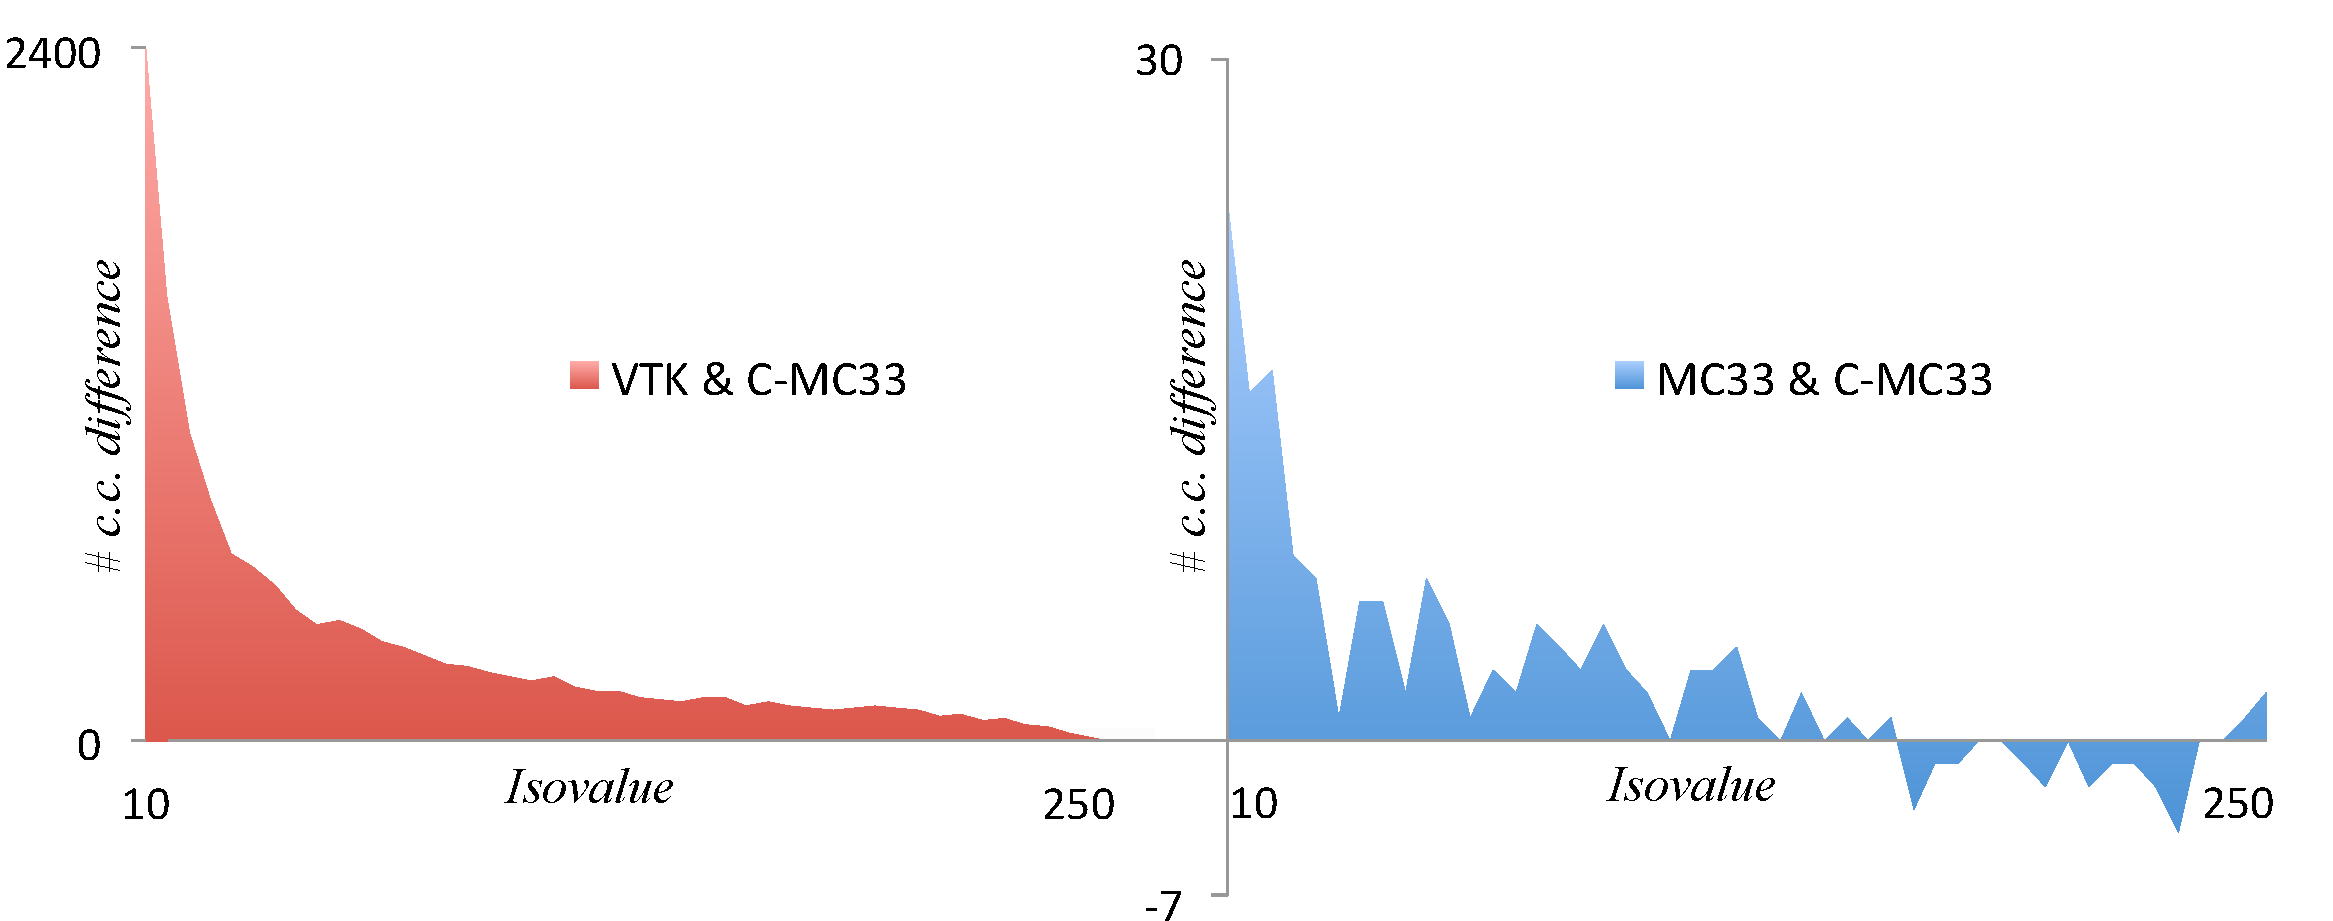
\includegraphics[width=1\linewidth]{chapter4/figures/aneurism_cc_vtk.pdf}
       \caption{\label{fig:cc} The left plot shows the difference between the number of connected components extracted by VTK implementation of Marching Cubes and the number of connected components extracted by our \cmc{} implementation. The right plot shows the difference in the number of connected components but between the \mc{} and  \cmc{} implementations. Negative values indicate that the \cmc{} implementation generated more connected components.
Clearly, VTK generates more components that \cmc{}. \mc{} generates more components for most of the isovalues. }
\end{figure}

\section{Conclusion}
\label{conclusion}

In this chapter, we discussed in detail three issues with  the Marching Cubes 33 algorithm and one non-trivial issue with its implementation. 
We presented solutions for the issues raised and implement them into \cmc, a topologically correct version of \mc. In addition, we made our results reproducible so that the reader can easily study, explore, and use the results presented here for his or her own purpose. 

\begin{figure}[b]
     \centering
     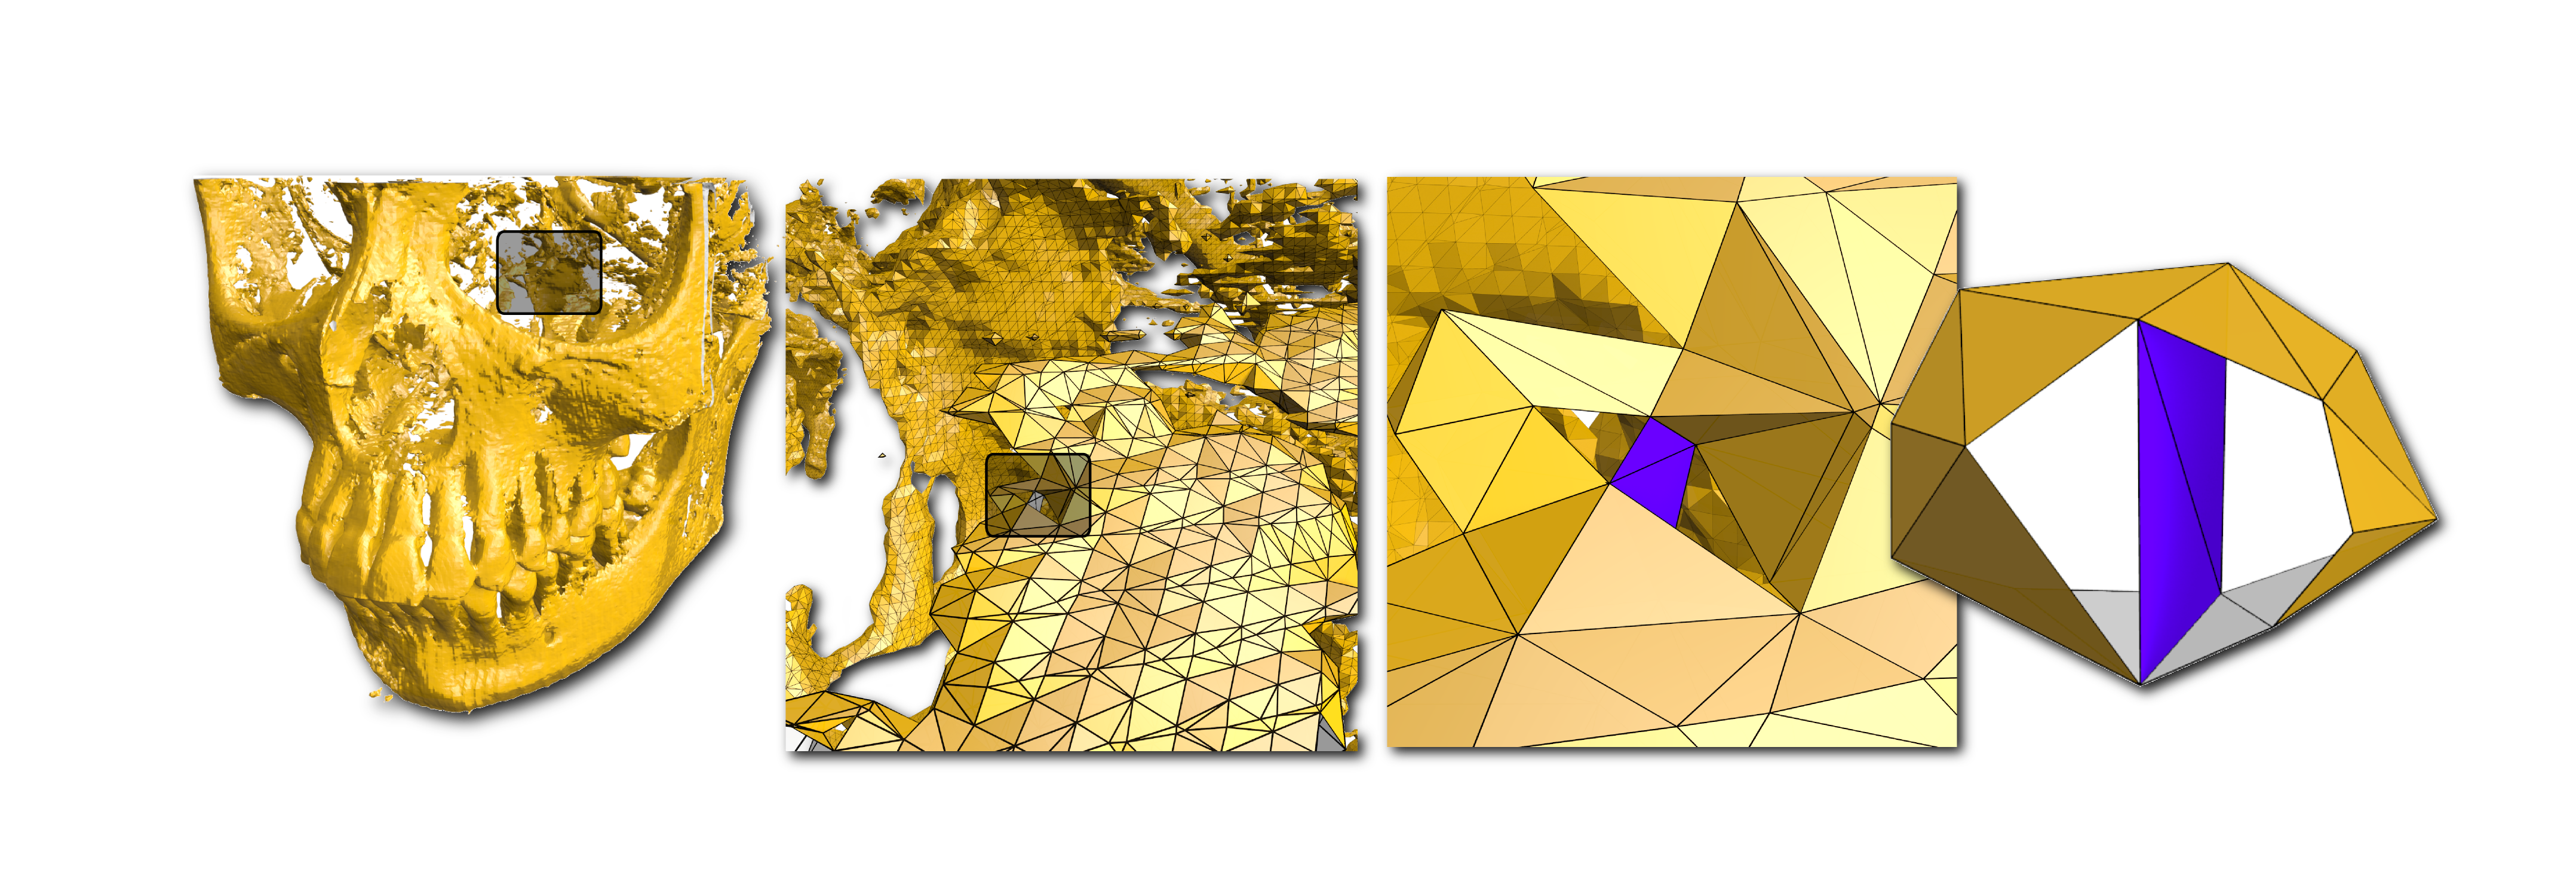
\includegraphics[width=0.9\linewidth]{chapter4/figures/skull.png}
     \caption{Skull dataset. The image shows a progressive zoom-in into the dataset in order to reveal non-manifold edges. The face containing the non-manifold edges is highlighted  in purple. The rightmost image is an isolated version of the case shown in the dataset, with a slightly different geometry for the sake of clarity. A non-manifold edge appeared six times in total for 50 distinct isosurfaces.}
     \label{fig:non-manifold-real-data}
\end{figure}
